% vim:autoindent:set textwidth=78:

\section{Utiliser des donn\'ees vecteurs}\label{label_workingvector}
%\index{vector layers|(}
\index{couches vecteur|(}

% when the revision of a section has been finalized, comment out the following line:
% \updatedisclaimer


%QGIS supports vector data in a number of formats, including those supported by the OGR library data provider plugin, such as ESRI shapefiles, \index{shapefiles}\index{ESRI!shapefiles}\index{SHP files} MapInfo MIF (interchange format)\index{MIF files}\index{MapInfo!MIF files} and MapInfo TAB (native format).\index{TAB files}\index{MapInfo!TAB files}
%You find a list of OGR supported vector formats in Appendix~\ref{appdx_ogr}.
QGIS g\`ere un grand nombre de formats vecteur, dont ceux g\'er\'es par l'extension de conversion de donn\'ees de la biblioth\`eque OGR, comme les formats shapefile ESRI,\index{shapefiles}\index{ESRI!shapefiles}\index{fichiers SHP} MapInfo MIF (format d'\'echange)\index{fichiers MIF}\index{MapInfo!fichiers MIF} et  MapInfo TAB (format natif).\index{fichiers TAB}\index{MapInfo!fichiers TAB}
Vous trouverez la liste des formats vectoriels support\'es par OGR dans l'Annexe~\ref{appdx_ogr}.

%QGIS also supports PostGIS\index{PostGIS}\index{PostgreSQL!PostGIS} layers in a PostgreSQL database using the PostgreSQL data provider plugin. Support for additional data types (eg. delimited text) is provided by additional data provider plugins.\index{delimited text}
QGIS g\`ere \'egalement les couches PostGIS\index{PostGIS}\index{PostgreSQL!PostGIS} des bases de donn\'ees PostgreSQL gr\^ace \`a l'extension ``fournisseur de donn\'ees'' PostgreSQL. La gestion d'autres types de donn\'ees (par exemple les donn\'ees texte d\'elimit\'ees) se fait gr\^ace \`a d'autres extensions ``fournisseur de donn\'ees''.\index{texte d\'elimit\'e}

%This section describes how to work with two common formats: ESRI shapefiles and PostGIS layers. Many of the features available in QGIS work the same regardless of the vector data source.
%This is by design and includes the identify, select, labeling and attributes functions.
Cette section d\'ecrit comment travailler avec deux des formats les plus communs : les shapefiles ESRI et les couches PostGIS. Beaucoup des fonctionnalit\'es de QGIS marchent, de par sa conception, de la m\^eme mani\`ere, quel que soit le format vecteur des donn\'ees sources. Il s'agit des fonctionnalit\'es d'identification, de s\'election, d'\'etiquetage et de gestion des attributs.

%Working with GRASS vector data is described in Section \ref{sec:grass}.
Le travail sur des couches vectorielles GRASS est d\'ecrit dans la Section \ref{sec:grass}.

%\subsection{ESRI Shapefiles}
%\index{vector layers!ESRI shapefiles}
%\index{shapefiles}
%\index{ESRI!shapefiles}
%\index{SHP files}
\subsection{Shapefiles ESRI}
\index{couches vecteur!shapefiles ESRI}
\index{shapefiles}
\index{ESRI!shapefiles}
\index{fichiers SHP}

%The standard vector file format used in QGIS is the ESRI Shapefile. It's support is provided by the OGR Simple Feature Library (\url{http://www.gdal.org/ogr/})\index{OGR}. A shapefile actually consists of a minimum of three files:\index{shapefile!format}
Le format de fichier vecteur standard utilis\'e par QGIS est le Shapefile ESRI. Il est g\'er\'e \`a travers la biblioth\`eque OGR Simple Feature  (\url{http://www.gdal.org/ogr/}) \index{OGR}. Un shapefile correspond en fait \`a un minimum de trois fichiers : \index{shapefile!format}

\begin{itemize}
%\item \filename{.shp} file containing the feature geometries.
%\item \filename{.dbf} file containing the attributes in dBase format.
%\item \filename{.shx} index file.
\item \filename{.shp} fichier contenant la g\'eom\'etrie des entit\'es.
\item \filename{.dbf} fichier contenant les attributs au format dBase.
\item \filename{.shx} fichier d'index.
\end{itemize}

%Ideally it comes with another file with a \filename{.prj} suffix, that contains the projection information for the shapefile. There can be more files belonging to a shapefile dataset. To have a closer look at this we recommend the technical specification for the shapefile format, that can be found at \url{http://www.esri.com/library/whitepapers/pdfs/shapefile.pdf}.\index{shapefile!specification}.
Dans l'id\'eal y est associ\'e un autre fichier ayant l'extension \filename{.prj} qui contient les informations sur le syst\`eme de coordonn\'ees utilis\'e pour le shapefile. Il peut y avoir encore d'autres fichiers associ\'es aux donn\'ees shapefile. Si vous souhaitez avoir plus de d\'etails nous vous recommandons de vous reporter aux sp\'ecifications techniques du format shapefile, qui se trouve notamment sur \url{http://www.esri.com/library/whitepapers/pdfs/shapefile.pdf}.\index{shapefile!sp\'ecifications}

%\subsubsection{Loading a Shapefile}\label{sec:load_shapefile}
\subsubsection{Charger un Shapefile}\label{sec:load_shapefile}
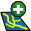
\includegraphics[width=0.7cm]{mActionAddNonDbLayer}
%To load a shapefile, start QGIS and click on the \toolbtntwo{mActionAddNonDbLayer}{Add a vector layer} toolbar button\index{shapefile!loading} or simply type \keystroke{V}. This same tool can be used to load any of the formats supported by the OGR library.
Pour charger un shapefile, lancer QGIS et cliquez sur \toolbtntwo{mActionAddNonDbLayer}{Ajouter une couche vecteur} dans la barre d'outil\index{shapefile!chargement} ou taper simplement \keystroke{V}. Ce m\^eme outil peut \^etre utilis\'e pour charger tous les formats g\'er\'es par la biblioth\`eque OGR.

%Clicking on the tool brings up a standard open file dialog (see Figure \ref{fig:openshapefile}) which allows you to navigate the file system and load
%a shapefile or other supported data source.
%The selection box \selectstring{Files of type}{\ldots} allows you to preselect some OGR supported file formats.
L'outil ouvre alors une fen\^etre de dialogue standard (voir Figure \ref{fig:openshapefile}) qui vous permet de naviguer dans les r\'epertoires et les fichiers et charger le shapefile ou tout autre format g\'er\'e.
La bo\^ite de s\'election \selectstring{Fichiers de type}{\ldots} vous permet de pr\'es\'electionner un format de fichier g\'er\'e par OGR.

%You can also select the Encoding type for the shapefile if desired.
Si vous le souhaitez,, vous pouvez \'egalement s\'electionner le type de codage du shapefile.

\begin{figure}[ht]
  \begin{center}
%  \caption{Open an OGR Supported Vector Layer Dialog \nixcaption}\label{fig:openshapefile}\smallskip
  \caption{Fen\^etre pour ouvrir une couche vecteur g\'er\'ee par OGR \nixcaption}\label{fig:openshapefile}\smallskip
  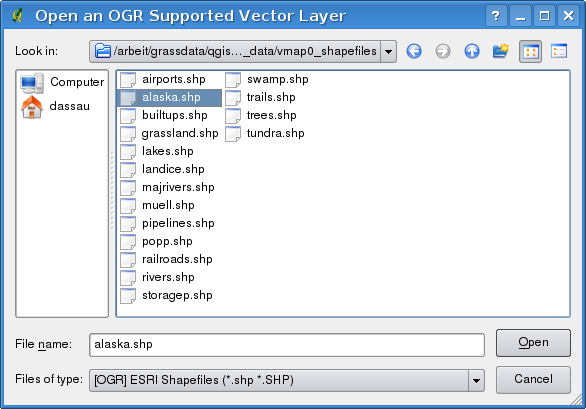
\includegraphics[clip=true, width=14cm]{shapefileopendialog}
\end{center}
\end{figure}

%Selecting a shapefile from the list and clicking \button{Open} loads it into QGIS. Figure \ref{fig:loadedshapefile} shows QGIS after loading the \filename{alaska.shp} file.
S\'electionner un shapefile dans la liste puis cliquer sur \button{Ouvrir} le charge dans QGIS. La figure \ref{fig:loadedshapefile} montre QGIS apr\`es avoir charg\'e le fichier \filename{alaska.shp}.

\begin{figure}[ht]
  \begin{center}
  %\caption{QGIS with Shapefile of Alaska loaded \nixcaption}\label{fig:loadedshapefile}\smallskip
  \caption{QGIS avec le Shapefile de l'Alaska charg\'e \nixcaption}\label{fig:loadedshapefile}\smallskip
  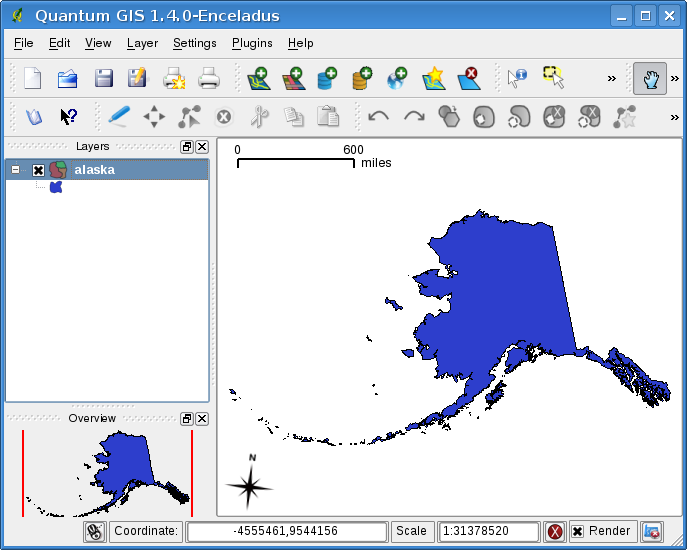
\includegraphics[clip=true, width=16cm]{shapefileloaded}
\end{center}
\end{figure}

%\begin{Tip}\caption{\textsc{Layer Colors}}
\begin{Tip}\caption{\textsc{Couleurs de couches}}
%\qgistip{When you add a layer to the map, it is assigned a random color. When adding more than one layer at a time, different colors are assigned to each layer.}
\qgistip{Quand vous ajoutez une couche sur une carte, une couleur al\'eatoire lui est assign\'ee. En ajoutant plusieurs couches en une fois, diff\'erentes couleurs sont assign\'ees \`a chacune des couches.}
\end{Tip}

%Once loaded, you can zoom around the shapefile using the map navigation tools.
%To change the symbology of a layer, open the \dialog{Layer Properties} dialog by double clicking on the layer name or by right-clicking on the name in the legend and choosing \dropmenuopt{Properties} from the popup menu. See Section \ref{sec:symbology} for more information on setting symbology of vector layers.
Une fois charg\'ee, vous pouvez zoomer sur le shapefile en utilisant les outils de navigation sur la carte.
Pour changer la symbologie d'une couche, ouvrez la fen\^etre \dialog{Propri\'et\'es de la Couche} en double-cliquant sur le nom de la couche ou en faisant un clic droit sur son nom dans la l\'egende et en choisissant \dropmenuopt{Propri\'et\'es} dans le menu qui apparait. Pour plus de d\'etails sur les param\`etres de la symbologie des couches vectorielles, r\'ef\'erez-vous \`a la Section \ref{sec:symbology}.

%\subsubsection{Improving Performance}
\subsubsection{Am\'eliorer les performances}

%To improve the performance of drawing a shapefile, you can create a spatial index. A \index{spatial index!shapefiles} spatial index will improve the  speed of both zooming and panning. Spatial indexes used by QGIS have a \filename{.qix} extension.
Pour am\'eliorer les performances de dessin d'un shapefile, vous pouvez cr\'eer un index spatial. Un \index{index spatial!shapefiles} index spatial am\'eliorera \`a la fois la vitesse d'ex\'ecution du zoom et du d\'eplacement panoramique. Les index spatiaux utilis\'es par QGIS ont une extension \filename{.qix}.

%Use these steps to create the index:
Voici les \'etapes de cr\'eation d'un index spatial :

\begin{itemize}
%\item Load a shapefile.
\item Chargez un shapefile
%\item Open the \dialog{Layer Properties} dialog by double-clicking on the shapefile name in the legend or by right-clicking and choosing \dropmenuopt{Properties} from the popup menu.
\item Ouvrez la fen\^etre \dialog{Propri\'et\'es de la Couche} en double-cliquant sur le nom de la couche dans la l\'egende ou en faisant un clic droit et en choisissant \dropmenuopt{Propri\'et\'es} dans le menu qui apparait.
%\item In the tab \tab{General} click the \button{Create Spatial Index} button.
\item Dans l'onglet \tab{G\'en\'eral}, cliquez sur le bouton \button{Cr\'eez un index spatial}.
\end{itemize}

%\subsubsection{Loading a MapInfo Layer}
%\index{vector layers!MapInfo}
\subsubsection{Charger une couche MapInfo}
\index{couches vecteur!MapInfo}

%To load a MapInfo layer, click on the \toolbtntwo{mActionAddNonDbLayer}{Add a vector layer} toolbar bar button or type \keystroke{V}, change the file type filter to \selectstring{Files of Type}{[OGR] MapInfo (*.mif *.tab *.MIF *.TAB)} and select the layer you want to load.
Pour charger une couche MapInfo, cliquez sur \toolbtntwo{mActionAddNonDbLayer}{Ajouter une couche vecteur} dans la barre d'outils ou tapez \keystroke{V}, changez le type de filtre pour \selectstring{Fichiers de type}{[OGR] MapInfo (*.mif *.tab *.MIF *.TAB)} et s\'electionnez la couche que vous souhaitez charger.

%\subsubsection{Loading an ArcInfo Coverage}
%\index{vector layers!ArcInfo Coverage}
\subsubsection{Charger une couverture ArcInfo}
\index{couches vecteur!couverture ArcInfo}

%Loading an ArcInfo coverage is done using the same method as with a shapefiles and MapInfo layers. Click on the \toolbtntwo{mActionAddNonDbLayer}{Add a vector layer} toolbar button or type \keystroke{V} to open the \dialog{Open on OGR Supported Vector Layer} dialog and change the file type filter to \selectstring{Files of Type}{All files (*.*)}. Navigate to the coverage directory and select one of the following files (if present in your coverage):
Charger une couverture ArcInfo se fait de la m\^eme mani\`ere que pour les couches shapefile ou MapInfo. Cliquez sur \toolbtntwo{mActionAddNonDbLayer}{Ajouter une couche vecteur} dans la barre d'outils ou tapez \keystroke{V} pour ouvrir la fen\^etre \dialog{Ouvrir une couche de vecteur g\'er\'ee par OGR} et changer le type de filtre pour \selectstring{Fichiers de type}{All files (*.*)}. Allez au r\'epertoire de votre couverture et s\'electionnez l'un des fichiers suivants (s'ils sont pr\'esents pour votre couverture) :

\begin{itemize}
%\item \filename{.lab} - to load a label layer (polygon labels or standing points).
\item \filename{.lab} - Pour charger une couche d'\'etiquettes (polygones d'\'etiquettes ou points)
%\item \filename{.cnt} - to load a polygon centroid layer
\item \filename{.cnt} - Pour charger une couche de centro"ides de polygones
%\item \filename{.arc} - to load an arc (line) layer.
\item \filename{.arc} - Pour charger une couche d'arcs (lignes)
%\item \filename{.pal} - to load a polygon layer.
\item \filename{.pal} - Pour charger une couche de polygones.
\end{itemize}

%\subsection{PostGIS Layers}
\subsection{Couches PostGIS}
%\index{vector layers!PostGIS|see{PostGIS}}
\index{couches vecteur!PostGIS|voir{PostGIS}}
%\index{PostGIS!layers}
\index{PostGIS!couches}
\label{label_postgis}

%PostGIS layers are stored in a PostgreSQL database. The advantages of PostGIS are the spatial indexing, filtering and query capabilities it provides. Using PostGIS, vector functions such as select and identify work more accurately than with OGR layers in QGIS.
Les couches PostGIS sont stock\'ees dans une base de donn\'ees PostgreSQL. Les avantages de PostGIS sont les possibilit\'es d'indexation spatiale, de filtre et de requ\^ete qu'il fournit. En utilisant PostGIS, les fonctions vecteur telles que la s\'election ou l'identification fonctionnent avec plus d'exactitude qu'avec les couches OGR dans QGIS.

%To use PostGIS layers you must:\index{PostgreSQL!loading layers}
Pour charger une couche PostGIS, vous devez :\index{PostgreSQL!charger des couches}

\begin{itemize}
%\item Create a stored connection in QGIS to the PostgreSQL database (if one is not already defined).\index{PostgreSQL!connection}
\item Dans QGIS, cr\'eez une connexion enregistr\'ee \`a une base de donn\'ees PostgreSQL (si elle n'a pas \'et\'e encore d\'efini).\index{PostgreSQL!connexion}
%\item Connect to the database.
\item Connectez-vous \`a la base de donn\'ees.
%\item Select the layer to add to the map.
\item S\'electionnez la couche \`a ajouter \`a la carte.
%\item Optionally provide a SQL \usertext{where} clause to define which features to load from the layer.
\item En option vous pouvez fournir une clause SQL \usertext{where} pour d\'efinir les entit\'es de la couche \`a charger.
%\item Load the layer.
\item Charger la couche.
\end{itemize}

%\subsubsection{Creating a stored Connection}\index{PostgreSQL!connection}\label{sec:postgis_stored}
\subsubsection{Cr\'eer une connexion enregistr\'ee}\index{PostgreSQL!connexion}\label{sec:postgis_stored}

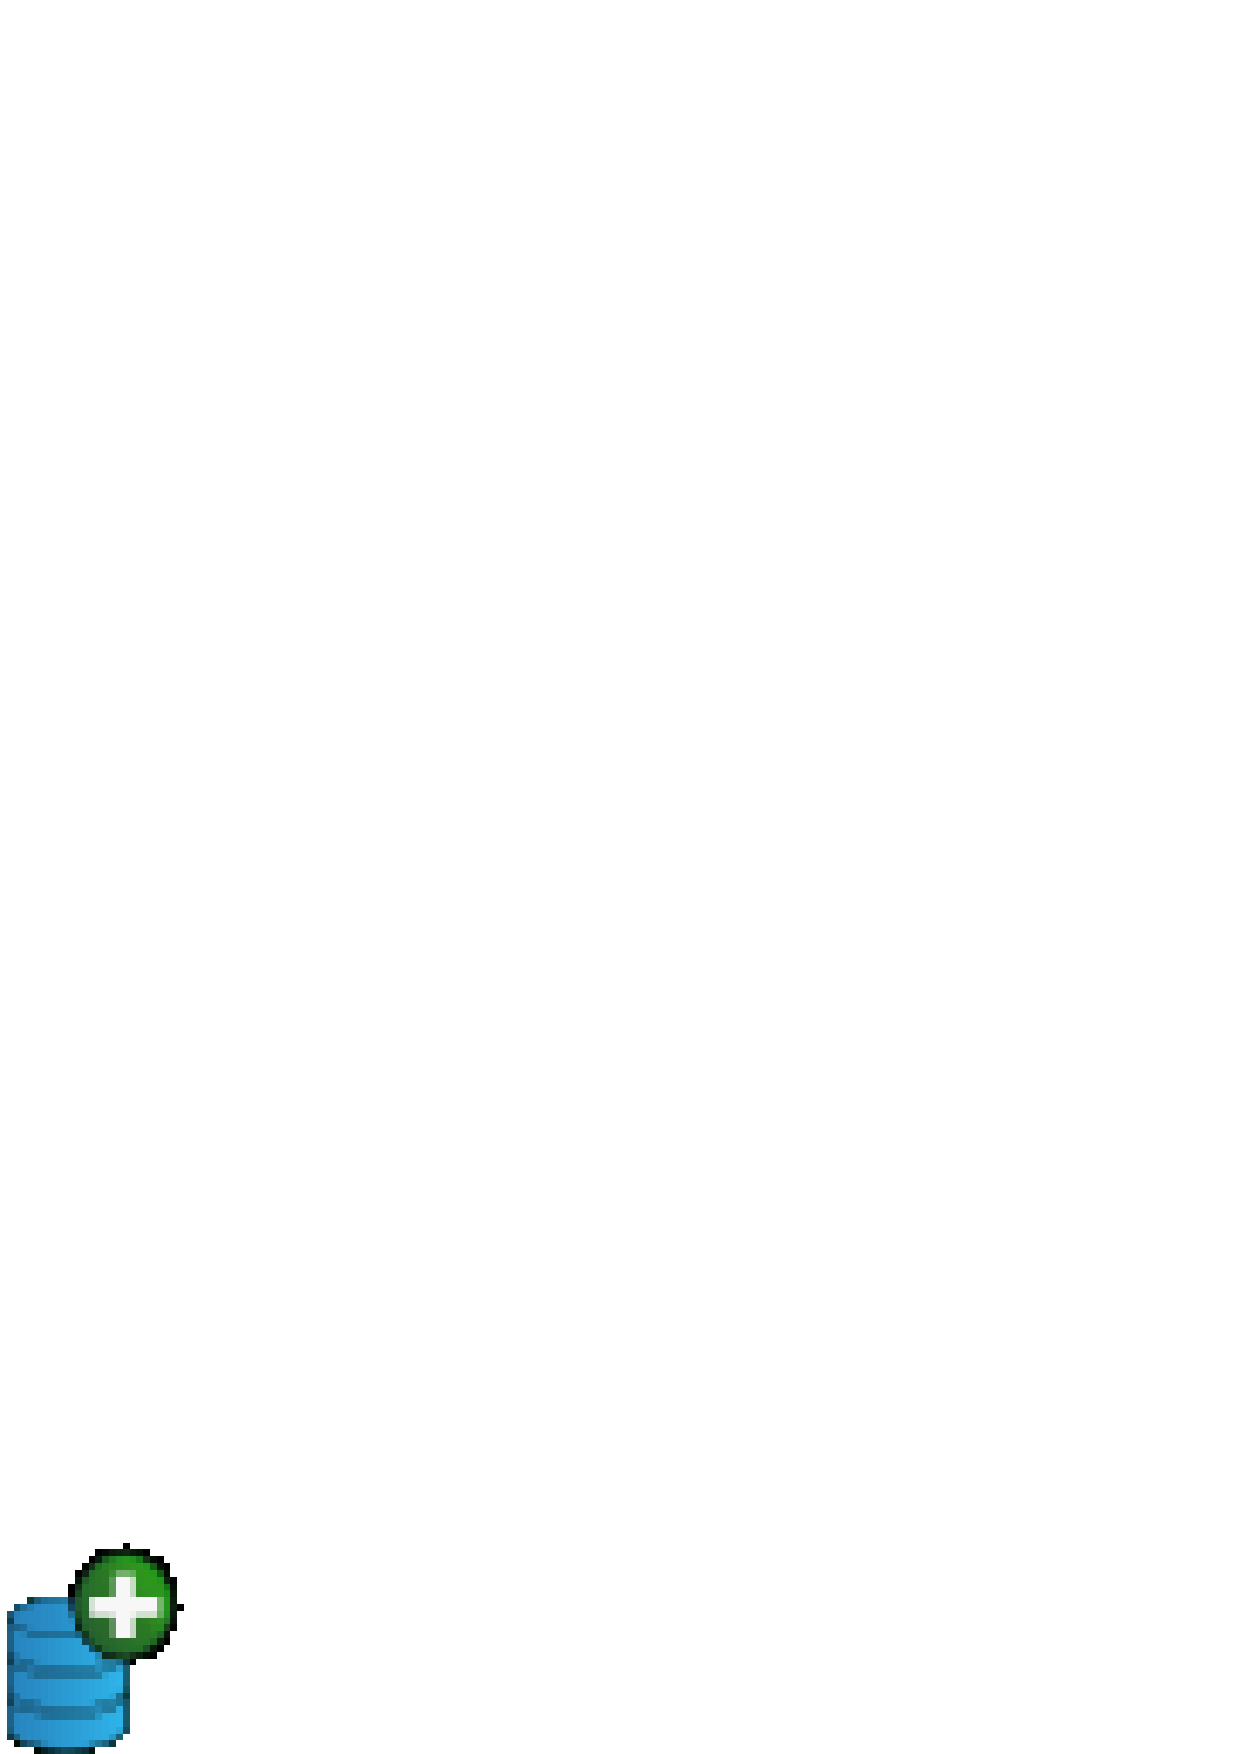
\includegraphics[width=0.7cm]{mActionAddLayer}
%The first time you use a PostGIS data source, you must create a connection to the PostgreSQL database that contains the data. Begin by clicking on the \toolbtntwo{mActionAddLayer}{Add a PostGIS Layer} toolbar button, selecting the \dropmenuopttwo{mActionAddLayer}{Add a PostGIS Layer...} option from the \mainmenuopt{Layer} menu or typing \keystroke{D}.
La premi\`ere fois que utilisez une source de donn\'ees PostGIS, vous devez cr\'eer une connexion \`a une base de donn\'ees PostgreSQL qui contient les donn\'ees. Commencez par cliquer sur le bouton \toolbtntwo{mActionAddLayer}{Ajouter une couche PostGIS} de la barre d'outils ou s\'electionner l'option \dropmenuopttwo{mActionAddLayer}{Ajouter une couche PostGIS...} dans le menu \mainmenuopt{Couche} ou taper \keystroke{D}.
%The \dialog{Add PostGIS Table(s)} dialog will be displayed. To access the connection manager\index{PostgreSQL!connection manager}, click on the \button{New} button to display the \dialog{Create a New PostGIS Connection} dialog. The parameters required for a connection are shown in table \ref{tab:postgis_connection_parms}.
La fen\^etre \dialog{Ajouter une ou plusieurs tables PostGIS} appara\^it. Pour acc\'eder au gestionnaire de connexion\index{PostgreSQL!gestionnaire de connexion}, cliquez sur le bouton \button{Nouveau} pour faire apparaitre la fen\^etre \dialog{Cr\'eer une nouvelle connexion PostGIS}. Les param\`etres requis pour la connexion sont pr\'esent\'es dans le tableau\ref{tab:postgis_connection_parms}.

\begin{table}[ht]\index{PostgreSQL!connection parameters}
\centering
%\caption{PostGIS Connection Parameters}\label{tab:postgis_connection_parms}\medskip
\caption{Param\`etres de connexion PostGIS}\label{tab:postgis_connection_parms}\medskip
\begin{tabular}{|l|p{5in}|}
%\hline Name & A name for this connection. Can be the same as \textsl{Database}.\\
\hline Nom & Un nom pour cette connexion. Il peut \^etre identique \`a \textsl{Base de donn\'ees}.\\
%\hline Host \index{PostgreSQL!host} & Name of the database host. This must be a resolvable host name the same as would be used to open a telnet connection or ping the host. If the database is on the same computer as QGIS, simply enter 'localhost' here.\\
\hline H\^ote \index{PostgreSQL!host} & Nom pour l'h\^ote de la base de donn\'ees. Il doit s'agir d'un nom existant, car il sera utilis\'e pour ouvrir une connexion Telnet ou interroger l'h\^ote. Si la base de donn\'ees est sur le m\^eme ordinateur que QGIS, mettez simplement 'localhost'. \\
%\hline Database \index{PostgreSQL!database} & Name of the database.\\
\hline Base de donn\'ees \index{PostgreSQL!database} & Nom de la base de donn\'ees.\\
%\hline Port \index{PostgreSQL!port}& Port number the PostgreSQL database server listens on. The default port is 5432.\\
\hline Port \index{PostgreSQL!port}& Num\'ero de port que le serveur de base de donn\'ees PostgreSQL \'ecoute. Le port par d\'efaut est 5432.\\
%\hline Username \index{PostgreSQL!username}& User name used to login to the database.\\
\hline Nom d'utilisateur \index{PostgreSQL!username} & Nom d'utilisateur utilis\'e pour se connecter \`a la base de donn\'ees.\\
%\hline Password \index{PostgreSQL!password}& Password used with \textsl{Username} to connect to the database.\\
\hline Mot de passe \index{PostgreSQL!password} & Mot de passe utilis\'e avec le \textsl{Nom d'utilisateur} pour se connecter \`a la base de donn\'ees.\\
\hline
\end{tabular}
\end{table}

%Optional you can activate follwing checkboxes:
Vous pouvez \'egalement activer les options suivantes :

\begin{itemize}
%\item \checkbox{Save Password}
\item \checkbox{Sauvegarder le mot de passe}
%\item \checkbox{Only look in the geometry\_columns table}
\item \checkbox{Uniquement regarder la table geometry\_columns}
%\item \checkbox{Only look in the 'public' schema}
\item \checkbox{Uniquement regarder dans le sch\'ema 'public'}
\end{itemize}

%Once all parameters and options are set, you can test the connection by clicking on the \button{Test Connect} button\index{PostgreSQL!connection!testing}.
Une fois que tous les param\`etres et les options sont d\'efinis, vous pouvez tester la connexion en cliquant que le bouton  \button{Test de connexion}\index{PostgreSQL!connexion!test}.

%\begin{Tip}\caption{\textsc{QGIS User Settings and Security}}\index{settings}\index{security}
\begin{Tip}\caption{\textsc{Param\`etres utilisateur de QGIS et S\'ecurit\'e}}\index{param\`etres}\index{s\'ecurit\'e}
%\qgistip{Your customized settings for QGIS are stored based on the operating system. \nix, the settings are stored in your home directory in \filename{.qt/qgisrc}. \win, the settings are stored in the registry. Depending on your computing environment, storing passwords in your QGIS settings may be a security risk.}
\qgistip{Vos param\`etres personnalis\'es pour QGIS sont stock\'es diff\'eremment selon le syst\`eme d'exploitation. \nix, les param\`etres sont stock\'es dans votre r\'epertoire home dans \filename{.qt/qgisrc}. \win, les param\`etres sont stock\'es dans la base de registre. Selon votre environnement informatique, stocker vos mots de passe dans vos param\`etres QGIS peut pr\'esenter des risques vis-\`a-vis de la s\'ecurit\'e.}
\end{Tip}

%\subsubsection{Loading a PostGIS Layer}\index{PostgreSQL!loading layers}
\subsubsection{Charger une couche PostGIS}\index{PostgreSQL!charger des couches}

%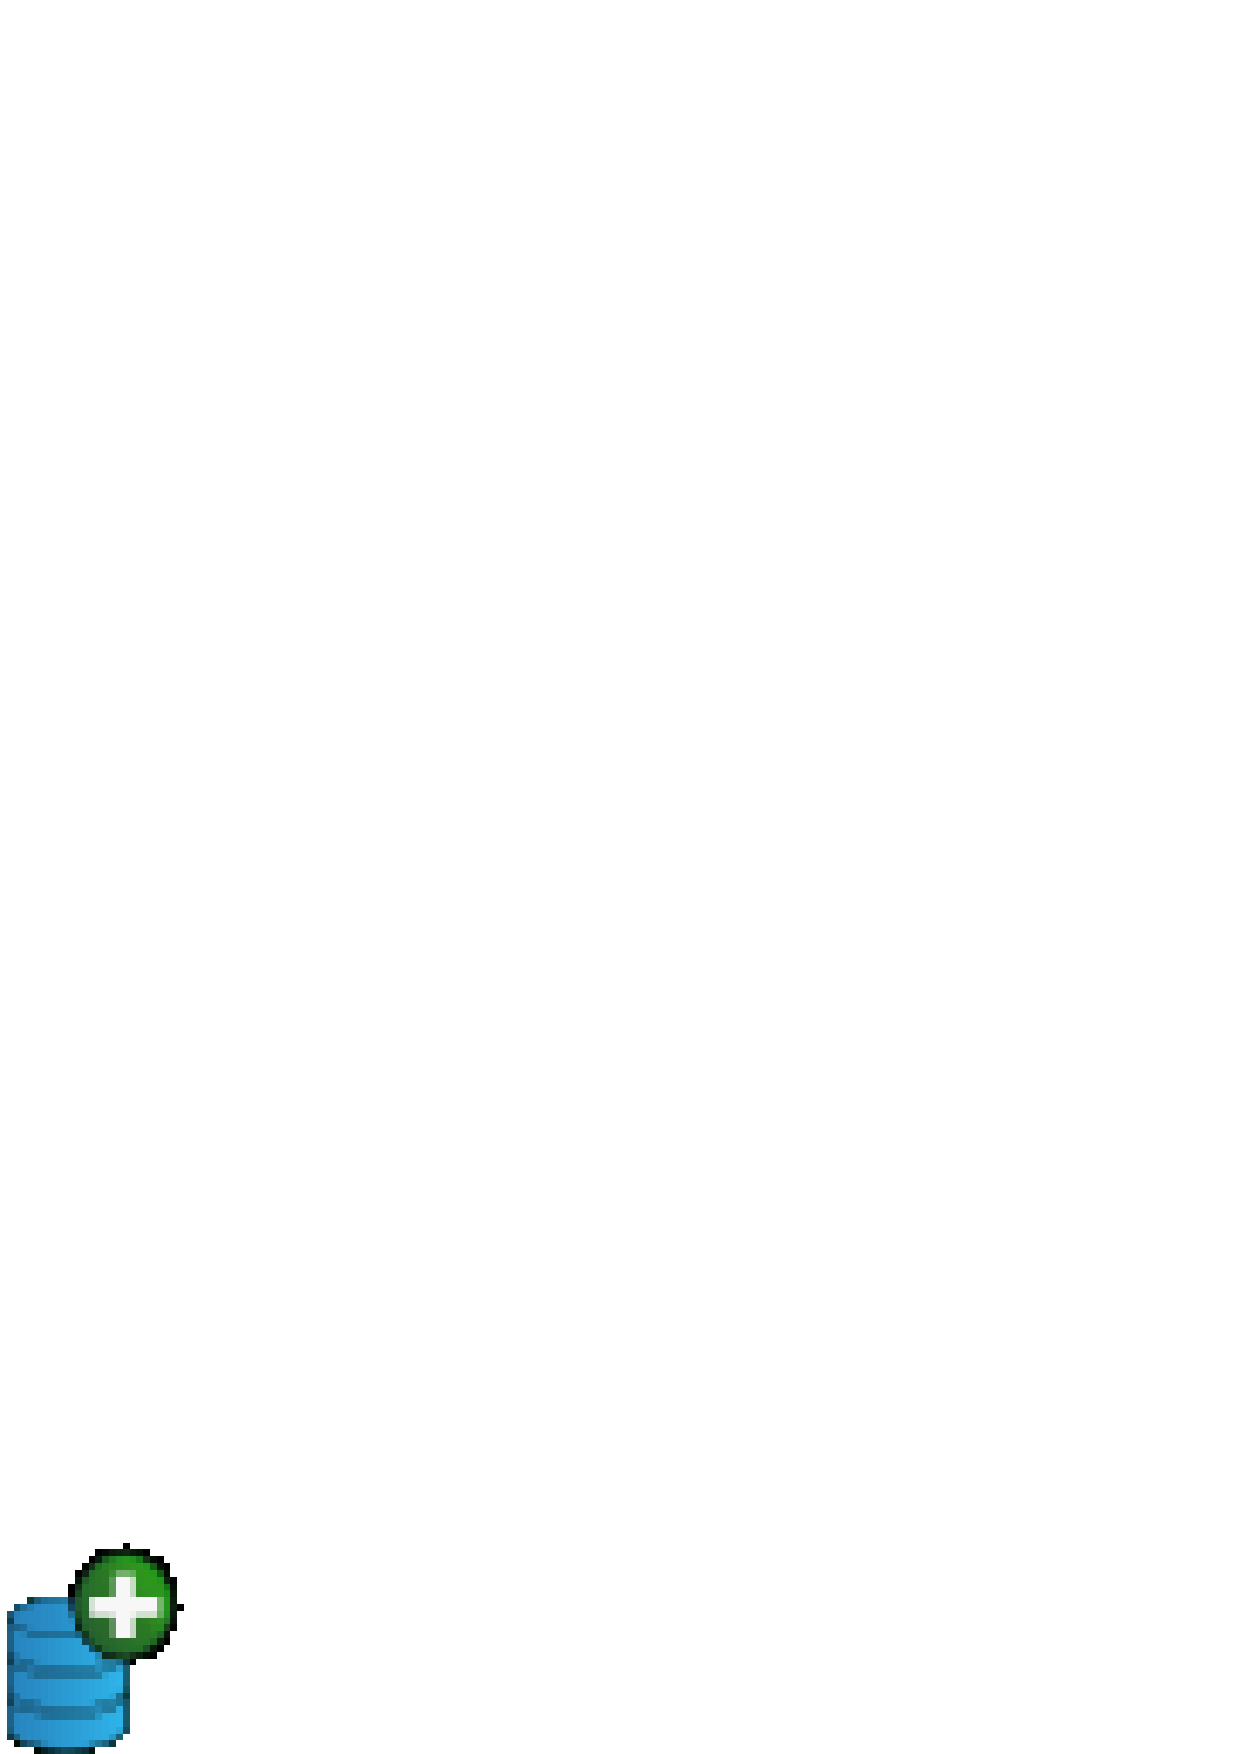
\includegraphics[width=0.7cm]{mActionAddLayer} Once you have one or more connections defined, you can load layers from the PostgreSQL database. Of course this requires having data in PostgreSQL. See Section \ref{sec:loading_postgis_data} for a discussion on importing data into the database.
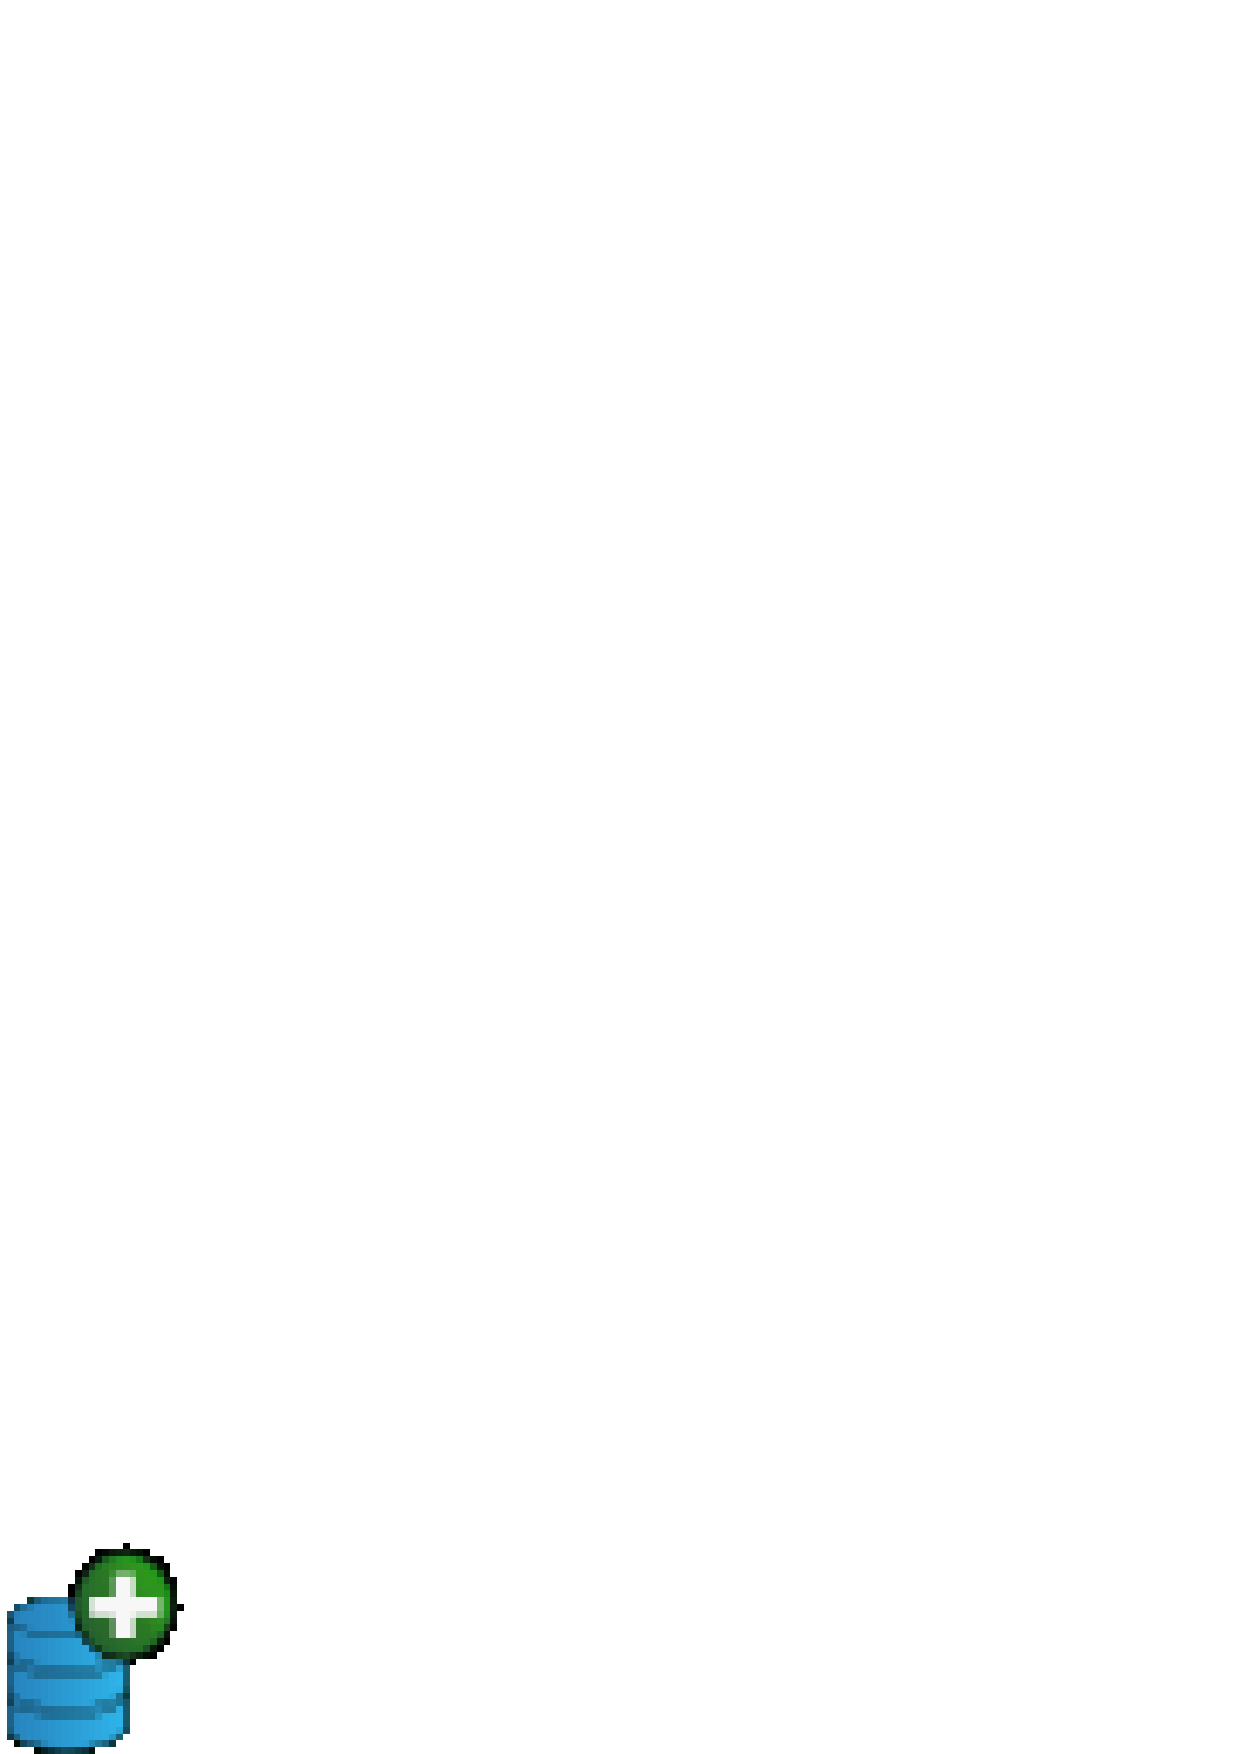
\includegraphics[width=0.7cm]{mActionAddLayer} Une fois une ou plusieurs connexions d\'efinies, vous pouvez charger des couches de la base de donn\'ees PostgreSQL. Bien s\^ur, cela n\'ecessite d'avoir des donn\'ees dans PostgreSQL. R\'ef\'erez-vous \`a la Section \ref{sec:loading_postgis_data} pour plus de d\'etails concernant l'importation de donn\'ees dans la base de donn\'ees.

%To load a layer from PostGIS, perform the following steps:
Pour charger une couche PostGIS, suivez ces \'etapes :

\begin{itemize}
%\item If the \dialog{Add PostGIS Table(s)} dialog is not already open, click on the \toolbtntwo{mActionAddLayer}{Add a PostGIS Layer} toolbar button.
\item Si la fen\^etre \dialog{Ajouter une ou plusieurs tables PostGIS} n'est pas ouverte, cliquez sur le bouton \toolbtntwo{mActionAddLayer}{Ajouter une couche PostGIS} de la barre d'outils.
%\item Choose the connection from the drop-down list and click \button{Connect}.
\item Choisissez la connexion dans la liste d\'eroulante et cliquez sur \button{Connecter}.
%\item Find the layer you wish to add in the list of available layers.
\item Trouvez la couche que vous souhaitez ajouter dans la liste des couches disponibles.
%\item Select it by clicking on it. You can select multiple layers by holding down the \keystroke{shift} key while clicking. See Section \ref{sec:query_builder} for information on using the PostgreSQL Query Builder to further define the layer.
\item S\'electionnez la en cliquant dessus. Vous pouvez s\'electionner plusieurs couches en gradant la touche \keystroke{shift} enfonc\'ee quand vous cliquez. R\'ef\'erez-vous \`a la Section \ref{sec:query_builder} pour plus d'informations sur l'utilisation du Constructeur de requ\^ete de PostgreSQL pour mieux d\'efinir la couche.
%\item Click on the \button{Add} button to add the layer to the map.
\item Cliquez sur le bouton \button{Ajouter} pour ajouter la couche \`a la carte.
\end{itemize}

%\begin{Tip}\caption{\textsc{PostGIS Layers}}
\begin{Tip}\caption{\textsc{Couches PostGIS}}
%\qgistip{Normally a PostGIS layer is defined by an entry in the geometry\_columns table. From version \OLD % should be 0.9.0 on, QGIS can load layers that do not have an entry in the geometry\_columns table. This includes both tables and views. Defining a spatial view provides a powerful means to visualize your data. Refer to your PostgreSQL manual for information on creating views.}
\qgistip{Normalement, une couche PostGIS est d\'efinie par une entr\'ee dans la table geometry\_columns. Depuis la version 0.11.0, QGIS peut charger des couches qui n'ont pas d'entr\'ee dans la table geometry\_columns. Ceci concerne aussi bien les tables que les vues. D\'efinir une vue spatiale fournit un moyen puissant pour visualiser vos donn\'ees. R\'ef\'erez-vous \`a votre manuel PostgreSQL pour plus d'informations sur la cr\'eation des vues.}
\end{Tip}

%\subsubsection{Some details about PostgreSQL layers}\label{sec:postgis_details}
%\index{PostgreSQL!layer details}
\subsubsection{Quelques \'el\'ements de d\'etail \`a propos des couches PostgreSQL}\label{sec:postgis_details}
\index{PostgreSQL!d\'etails sur les couches}

%This section contains some details on how QGIS accesses PostgreSQL layers. Most of the time QGIS should simply provide you with a list of database tables that can be loaded, and load them on request. However, if you have trouble loading a PostgreSQL table into QGIS, the information below may help you understand any QGIS messages and give you direction on changing the PostgreSQL table or view definition to allow QGIS to load it.
Cette sections contient quelques d\'etails sur la mani\`ere dont QGIS acc\`ede aux couches PostgreSQL. La plupart du temps, QGIS devrait simplement fournir une liste de tables de base de donn\'ees qui peuvent \^etre charg\'ees et les charge \`a la demande. Cependant, si vous avez des probl\`emes pour charger une table PostgreSQL dans QGIS, les informations donn\'ees ci-dessous peuvent vous aider \`a comprendre les messages de QGIS et vous donnez une indication sur comment changer la table ou la vue PostgreSQL pour qu'elle se charge dans QGIS.

%QGIS requires that PostgreSQL layers contain a column that can be used as a unique key for the layer. For tables this usually means that the table needs a primary key, or a column with a unique constraint on it. QGIS additionally requires that this column be of type int4 (an integer of size 4 bytes). If a table lacks these items, the oid column will be used instead. Performance will be improved if the column is indexed (note that primary keys are automatically indexed in PostgreSQL).
QGIS demande que les couches PostgreSQL aient un champ qui peut \^etre utilis\'e comme cl\'e unique pour la couche. Pour les tables, cela signifie qu'elles doivent avoir une cl\'e primaire ou un champ ayant une contrainte d'unicit\'e. De plus, QGIS impose que cette colonne soit de type int4 (un entier de 4 bites). Si une table ne respecte pas ces conditions, le champ oid sera utilis\'e \`a la place. Les performances seront am\'elior\'ees si le champ est index\'e (notez que les cl\'es primaires sont automatiquement index\'ees dans PostgreSQL).

%If the PostgreSQL layer is a view, the same requirements exists, but views don't have primary keys or columns with unique constraints on them. In this case QGIS will try to find a column in the view that is derived from a table column that is suitable. If one cannot be found, QGIS will not load the layer. If this occurs, the solution is to alter the view so that it does include a suitable column (a type of int4 and either a primary key or with a unique constraint, preferably indexed).
Si la couche PostgreSQL est une vue, les m\^emes conditions s'appliquent mais elles n'ont pas de cl\'e primaire ou de champ ayant une contrainte d'unicit\'e. Dans ce cas, QGIS essayera de trouver un champ de la vue issu d'un champ une table qui convienne. S'il ne peut pas en trouver, QGIS ne chargera pas la couche. Si cela arrive, la solution consiste \`a modifier la vue de telle sorte qu'elle inclut un champ qui convienne (de type int4 et ayant soit une cl\'e primaire soit une contrainte d'unicit\'e, de pr\'ef\'erence index\'ee).

%\subsubsection{Importing Data into PostgreSQL}\label{sec:loading_postgis_data}\index{PostGIS!SPIT!importing data}
\subsubsection{Importing Data into PostgreSQL}\label{sec:loading_postgis_data}\index{PostGIS!SPIT!importer des donn\'ees}

\minisec{shp2pgsql}
%Data can be imported into PostgreSQL using a number of methods. PostGIS includes a utility called \filename{shp2pgsql} that can be used to import shapefiles into a PostGIS enabled database. For example, to import a shapefile named \filename{lakes.shp} into a PostgreSQL database named \usertext{gis\_data}, use the following command:
De multiples m\'ethodes existent pour importer des donn\'ees dans PostgreSQL. PostGIS inclut un utilitaire nomm\'e \filename{shp2pgsql} qui peut \^etre utilis\'e pour importer des shapefiles dans des bases de donn\'ees disposant de PostGIS. Par exemple, pour importer le shapefile \filename{lakes.shp} dans une base de donn\'ees PostgreSQL nomm\'ee \usertext{gis\_data}, utiliser la commande suivante :

\begin{verbatim}
  shp2pgsql -s 2964 lakes.shp lakes_new | psql gis_data
\end{verbatim}

%This creates a new layer named \usertext{lakes\_new} in the \usertext{gis\_data} database. The new layer will have a spatial reference identifier (SRID) of 2964. See Section \ref{label_projections} for more information on spatial reference systems and projections.
Ceci cr\'ee une nouvelle couche nomm\'ee \usertext{lakes\_new} dans la base de donn\'ees usertext{gis\_data}. La nouvelle couche aura l'identifiant de r\'ef\'erence spatiale (SRID) 2964. R\'ef\'erez-vous \`a la Section \ref{label_projections} pour plus d'informations sur les syst\`emes de r\'ef\'erence spatiale et les projections.
\begin{Tip}
%\caption{\textsc{Exporting datasets from PostGIS}\index{PostGIS!Exporting}}
\caption{\textsc{Exporter des jeux de donn\'ees depuis PostGIS}\index{PostGIS!Exporter}}
%\qgistip{Like the import-tool \filename{shp2pgsql} there is also a tool to export PostGIS-datasets as shapefiles: \filename{pgsql2shp}. This is shipped within your PostGIS distribution.}
\qgistip{Comme l'outil d'importation \filename{shp2pgsql}, il y a \'egalement un outil d'exportation de jeux de donn\'ees PostGIS en shapefile : \filename{pgsql2shp}. Cet outil est inclus dans la distribution de PostGIS.}
\end{Tip}

%\minisec{SPIT Plugin}
\minisec{Extension SPIT}
%
\includegraphics[width=0.7cm]{spiticon} QGIS comes with a plugin named SPIT (Shapefile to PostGIS Import Tool)\index{PostGIS!SPIT}. SPIT can be used to load multiple shapefiles at one time and includes support for schemas. To use SPIT, open the Plugin Manager from the \mainmenuopt{Plugins} menu, check the box next to the \checkbox{SPIT plugin} and click \button{OK}. The SPIT icon will be added to the plugin toolbar\index{PostGIS!SPIT!loading}.

\includegraphics[width=0.7cm]{spiticon} QGIS est distribu\'e avec une extension nomm\'ee SPIT (Shapefile to PostGIS Import Tool)\index{PostGIS!SPIT}. SPIT peut \^etre utilis\'e pour charger plusieurs shapefiles en une fois et inclut la gestion des sch\'emas. Pour utiliser SPIT, ouvrez le Gestionnaire d'extensions depuis le menu \mainmenuopt{Plugins}, cochez la case adjacente \`a \checkbox{SPIT plugin} et cliquez sur \button{OK}. L'ic\^one SPIT sera ajout\'ee \`a la barre d'outils\index{PostGIS!SPIT!charger}.

%To import a shapefile, click on the \toolbtntwo{spiticon}{SPIT} tool in the toolbar to open the \dialog{SPIT - Shapefile to PostGIS Import Tool} dialog. Select the PostGIS database you want to connect to and click on \button{Connect}. Now you can add one or more files to the queue by clicking on the \button{Add} button. To process the files, click on the \button{OK} button. The progress of the import as well as any errors/warnings will be displayed as each shapefile is processed.
Pour importer un shapefile, cliquez sur le bouton \toolbtntwo{spiticon}{SPIT} dans la barre d'outils pour ouvrir la fen\^etre \dialog{SPIT - Outil d'importation de Shapefile dans PostGIS}. S\'electionnez la base de donn\'ees \`a laquelle vous voulez vous connecter et cliquez sur le bouton \button{Connecter}. Vous pouvez alors ajouter un ou plusieurs fichiers \`a la liste en cliquant sur le bouton \button{Ajouter}. Pour traiter les fichiers, appuyez sur le bouton \button{OK}. La progression de l'importation aussi bien que les erreurs ou les alertes s'afficheront pour chaque shapefile.

%\begin{Tip}\caption{\textsc{Importing Shapefiles Containing PostgreSQL Reserved Words}}\index{PostGIS!SPIT!reserved words}
\begin{Tip}\caption{\textsc{Importer des shapefiles contenant des mots r\'eserv\'es de PostgreSQL}}\index{PostGIS!SPIT!mots r\'eserv\'es}
%\qgistip{If a shapefile is added to the queue containing fields that are reserved words in the PostgreSQL database a dialog will popup showing the status of each field. You can edit the field names\index{PostGIS!SPIT!editing field names} prior to import and change any that are reserved words (or change any other field names as desired). Attempting to import a shapefile with reserved words as field names will likely fail.}
\qgistip{Si un shapefile est ajout\'e \`a la liste et que des noms de champs correspondent \`a des mots r\'eserv\'es dans une base de donn\'ees PostgreSQL, une fen\^etre apparaitra et montrera le statut de chaque champ. Vous pouvez \'editer les noms des champs\index{PostGIS!SPIT!\'editer des noms de champ} avant l'importation et changer ceux qui correspondent \`a un mot r\'eserv\'e (ou faire les changements d\'esir\'es). Toute tentative d'importer un shapefile ayant un champ contenant un mot r\'eserv\'e devrait vraisemblablement \'echouer.}
\end{Tip}

\minisec{ogr2ogr}
%Beside \filename{shp2pgsql} and \filename{SPIT} there is another tool for feeding geodata in PostGIS: \filename{ogr2ogr}. This is part of your GDAL installation.
En plus de \filename{shp2pgsql} et \filename{SPIT}, un autre outil est fourni pour importer des donn\'ees g\'eographiques dans PostGIS : \filename{ogr2ogr}. Il est inclus dans GDAL.
%To import a shapefile into PostGIS, do the following:
Pour importer un shapefile dans PostGIS, tapez la commande suivante :
\begin{verbatim}
  ogr2ogr -f "PostgreSQL" PG:"dbname=postgis host=myhost.de user=postgres \
  password=topsecret" alaska.shp
\end{verbatim}

%This will import the shapefile \filename{alaska.shp} into the PostGIS-database \usertext{postgis} using the user \usertext{postgres} with the password \usertext{topsecret} on host \server{myhost.de}.
Ceci va importer le shapefile \filename{alaska.shp} dans la base de donn\'ees PostGIS \usertext{postgis} en utilisant l'utilisateur \usertext{postgres} avec le mot de passe \usertext{topsecret} sur l'h\^ote \server{myhost.de}.

%Note that OGR must be built with PostgreSQL to support PostGIS. You can see this by typing
Notez qu'OGR doit \^etre compil\'e avec PostgreSQL pour g\'erer PostGIS. Vous pouvez v\'erifier en tapant :
\begin{verbatim}
ogrinfo --formats | grep -i post
\end{verbatim}

%If you like to use PostgreSQL's \filename{COPY}-command instead of the default \filename{INSERT INTO} method you can export the following environment-variable (at least available on \nix and \osx):
Si vous pr\'ef\'erez utiliser la commande PostgreSQL \filename{COPY} au lieu de la m\'ethode par d\'efaut, \filename{INSERT INTO}, vous pouvez exporter la variable d'environnement suivante (au moins sur \nix et \osx) :
\begin{verbatim}
  export PG_USE_COPY=YES
\end{verbatim}

%\filename{ogr2ogr} does not create spatial indexes like \filename{shp2pgsl} does. You need to create them manually using the normal SQL-command \filename{CREATE INDEX} afterwards as an extra step (as described in the next section \ref{label_improve}).
\filename{ogr2ogr} ne cr\'ee pas d'index spatial comme le fait \filename{shp2pgsl}. Vous devez effectuer une \'etape suppl\'ementaire et le cr\'eer manuellement apr\`es en utilisant la commande SQL classique \filename{CREATE INDEX} (comme cela est d\'etaill\'e dans la section suivante \ref{label_improve}).

%\subsubsection{Improving Performance} \label{label_improve}
\subsubsection{Am\'eliorer les performances} \label{label_improve}

%Retrieving features from a PostgreSQL database can be time consuming, especially over a network. You can improve the drawing performance of PostgreSQL layers by ensuring that a \index{PostGIS!spatial index} spatial index exists on each layer in the database. PostGIS supports creation of a \index{PostGIS!spatial index!GiST} GiST (Generalized Search Tree) index to speed up spatial searches of the data.
R\'ecup\'erer des entit\'es depuis une base de donn\'ees PostgreSQL peut \^etre long, surtout par un r\'eseau. Vous pouvez am\'eliorer les performances de dessin de couches PostgreSQL en vous assurant qu'un \index{PostGIS!index spatial} index spatial existe pour chaque couche dans la base de donn\'ees. PostGIS g\`ere la cr\'eation d'un index \index{PostGIS!index spatial!GiST} GiST (Generalized Search Tree) pour acc\'el\'erer les recherches spatiales sur les donn\'ees.

%The syntax for creating a GiST\footnote{GiST index information is taken from the PostGIS documentation available at \url{http://postgis.refractions.net}} index is:
La syntaxe pour cr\'eer un index GiST\footnote{les informations de l'index GiST proviennent de la documentation de PostGIS disponible sur \url{http://postgis.refractions.net}} est la suivante :

\begin{verbatim}
    CREATE INDEX [indexname] ON [tablename]
      USING GIST ( [geometryfield] GIST_GEOMETRY_OPS );
\end{verbatim}

%Note that for large tables, creating the index can take a long time. Once the index is created, you should perform a \usertext{VACUUM ANALYZE}. See the PostGIS documentation \cite{PostGISweb} for more information.
Notez que pour de grandes tables, cr\'eer un index peut prendre du temps. Une fois cet index cr\'e\'e, vous devriez faire une \usertext{VACUUM ANALYZE}. R\'ef\'erez-vous \`a la documentation de \cite{PostGISweb} pour plus d'informations.

%The following is an example of creating a GiST index:
Voici un exemple de cr\'eation d'un index GiST :
\begin{verbatim}
gsherman@madison:~/current$ psql gis_data
Welcome to psql 8.3.0, the PostgreSQL interactive terminal.

Type:  \copyright for distribution terms
        \h for help with SQL commands
        \? for help with psql commands
        \g or terminate with semicolon to execute query
        \q to quit

gis_data=# CREATE INDEX sidx_alaska_lakes ON alaska_lakes
gis_data-# USING GIST (the_geom GIST_GEOMETRY_OPS);
CREATE INDEX
gis_data=# VACUUM ANALYZE alaska_lakes;
VACUUM
gis_data=# \q
gsherman@madison:~/current$
\end{verbatim}

%\subsection{The Vector Properties Dialog}\label{sec:vectorprops}
%\index{vector layers!properties dialog}
\subsection{La fen\^etre Propri\'et\'e des couches vecteur}\label{sec:vectorprops}
\index{couches vecteur!fen\^etre propri\'et\'e}

%The \dialog{Layer Properties} dialog for a vector layer provides information about the layer, symbology settings and labeling options. If your vector layer has been loaded from a PostgreSQL / PostGIS datastore, you can also alter the underlying SQL for the layer - either by hand editing the SQL on the \tab{General} tab or by invoking the \dialog{Query Builder} dialog on the \tab{General} tab. To access the \dialog{Layer Properties} dialog, double-click on a layer in the legend or right-click on the layer and select \dropmenuopt{Properties} from the popup menu.
La fen\^etre \dialog{Propri\'et\'es de la couche} pour une couche vecteur fournit des informations sur la couche, les param\`etres de repr\'esentation et les options d'\'etiquetage. Si votre couche a \'et\'e charg\'ee depuis une base PostgreSQL / PostGIS, vous pouvez \'egalement modifier la requ\^ete SQL d'appel de la couche, soit manuellement en \'editant le SQL dans l'onglet \tab{G\'en\'eral} soit en appelant la fen\^etre \dialog{Constructeur de requ\^ete} depuis l'onglet \tab{G\'en\'eral}. Pour acc\'eder \`a la fen\^etre \dialog{Propri\'et\'es de la couche}, double-cliquez sur la couche dans la l\'egende ou faites un clic droit sur la couche et s\'electionnez \dropmenuopt{Propri\'et\'es} dans le menu qui apparait.

\begin{figure}[H]
  \begin{center}
  %\caption{Vector Layer Properties Dialog \nixcaption}\label{fig:vector_symbology}\smallskip
  \caption{Fen\^etre Propri\'et\'es d'une couche vecteur \nixcaption}\label{fig:vector_symbology}\smallskip
  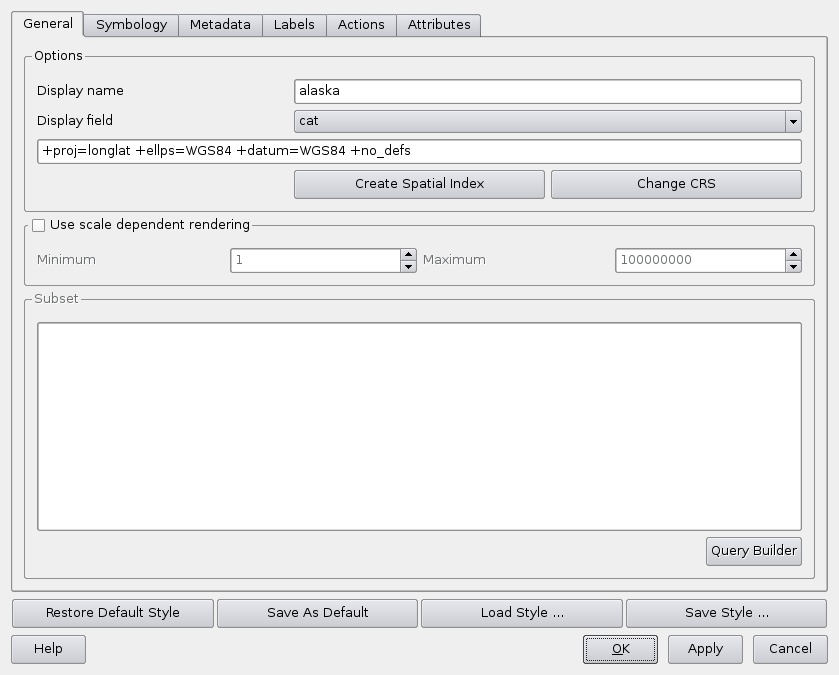
\includegraphics[clip=true, width=12cm]{vectorLayerSymbology}
\end{center}
\end{figure}

%\subsubsection{General Tab}\label{vectorgeneraltab}
\subsubsection{Onglet G\'en\'eral}\label{vectorgeneraltab}
%The \tab{General} tab is essentially like that of the raster dialog. It allows you to change the display name, set scale dependent rendering options, create a spatial index of the vector file (only for OGR supported formats and PostGIS) and view or change the projection of the specific vetor layer.
L'onglet \tab{G\'en\'eral} des couches vecteur est tr\`es proche de celui des couches raster. Il vous permet de changer le nom affich\'e, d\'efinir des rendus diff\'erents selon l'\'echelle, cr\'eer un index spatial du fichier vecteur (uniquement pour les formats g\'er\'es par OGR et PostGIS) et visualiser ou changer la projection de la couche.

%The \button{Query Builder} button allows you to create a subset of the features in the layer - but this button currently only is available when you open the attribute table and select the \button{Advanced ...} button.
Le bouton \button{Constructeur de requ\^ete} vous permet de cr\'eer un sous-ensemble d'entit\'e au sein de la couche - mais ce bouton de fonctionne actuellement que lorsque vous ouvrez la table attributaire et cliquez sur le bouton \button{Avanc\'ee...}.

%\subsubsection{Symbology Tab}\label{sec:symbology}
%\index{vector layers!symbology}
\subsubsection{Onglet Convention des signes}\label{sec:symbology}
\index{couches vecteur!symbologie}

%QGIS supports a number of symbology renderers to control how vector features are displayed. Currently the following renderers are available:
QGIS g\`ere diff\'erents types de repr\'esentation cartographique pour contr\^oler la mani\`ere pour les entit\'es vectorielles seront affich\'ees. Actuellement, voici les possibilit\'es :

\begin{description}
%\item[Single symbol] - a single style is applied to every object in the layer.\index{vector layers!renderers!single symbol}
\item[Symbole unique] - un style unique est appliqu\'e \`a tous les objets de la couche.\index{couches vecteur!rendus!symbole unique}
%\item[Graduated symbol] - objects within the layer are displayed with different symbols classified by the values of a particular field.\index{vector layers!renderers!graduated symbol}
\item[Symbole gradu\'e] - les objets de la couche sont repr\'esent\'es avec des symboles diff\'erents selon la valeur qu'ils ont dans un champ d\'efinit.\index{couches vecteur!rendus!symbole gradu\'e}
%\item[Continuous color] - objects within the layer are displayed with a spread of colours classified by the numerical values within a specified field.\index{vector layers!renderers!continuous color}
\item[Couleur continue] - les objets de la couche sont repr\'esent\'es avec une \'echelle de couleurs class\'ees selon les valeurs num\'eriques d'un champ d\'efinit.\index{couches vecteur!rendus!couleur continue}
%\item[Unique value] - objects are classified by the unique values within a specified field with each value having a different symbol.\index{vector layers!renderers!unique value}
\item[Valeur unique] - les objets sont class\'es par valeur unique dans un champ d\'efinit et \`a chaque valeur correspond un symbole diff\'erent.\index{couches vecteur!rendus!valeur unique}
\end{description}

%To change the symbology for a layer, simply double click on its legend entry and the vector \dialog{Layer Properties} dialog will be  shown.\index{symbology!changing}
Pour changer la symbologie d'une couche, double-cliquez simplement dessus dans la l\'egende et la fen\^etre de \dialog{Propri\'et\'es de la couche} appara\^itra.\index{symbologie!changer}

\begin{figure}[h]
\centering
\caption{Symbolizing-options \nixcaption}
  %\subfigure[Single symbol] {\label{subfig:single_symbol}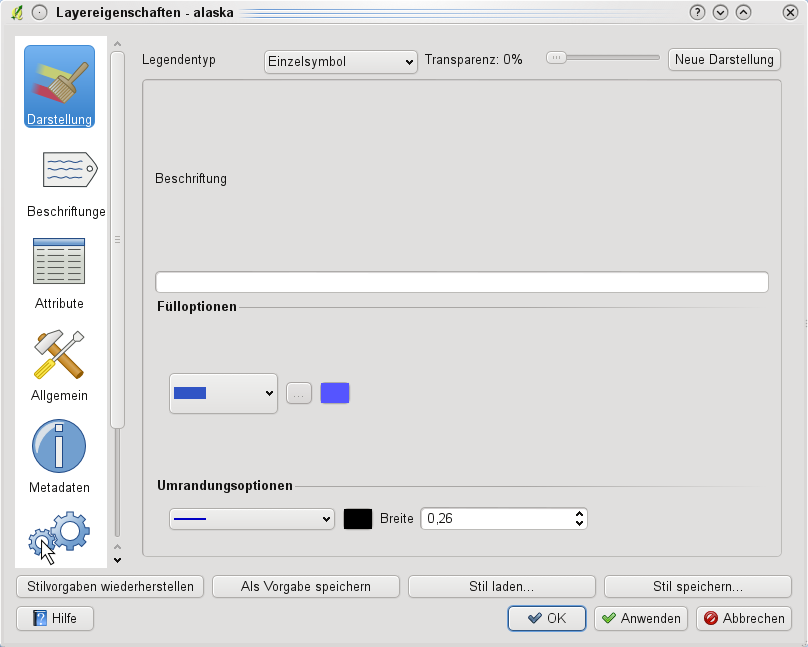
\includegraphics[clip=true, width=0.4\textwidth]{vectorClassifySingle}}\goodgap
  \subfigure[Symbole unique] {\label{subfig:single_symbol}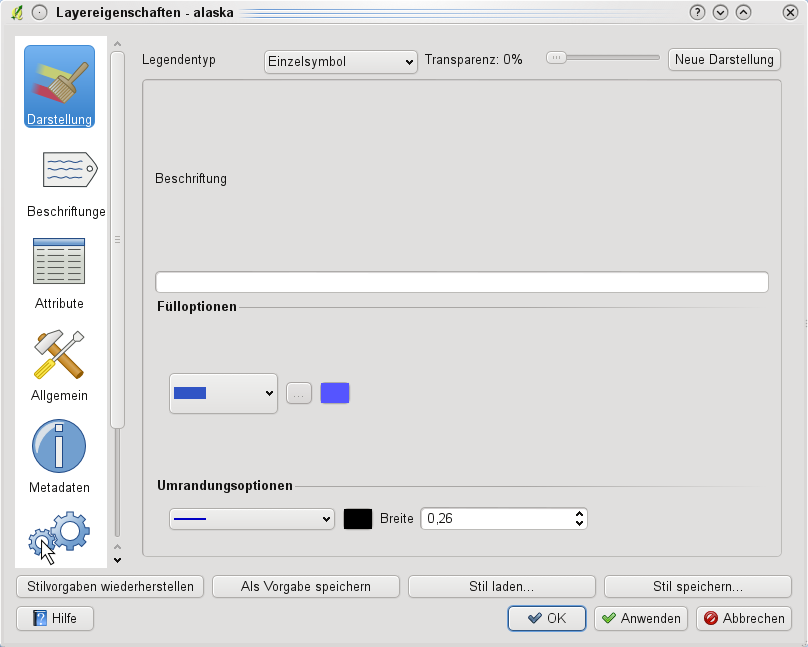
\includegraphics[clip=true, width=0.4\textwidth]{vectorClassifySingle}}\goodgap
  %\subfigure[Graduated symbol] {\label{subfig:graduated_symbol}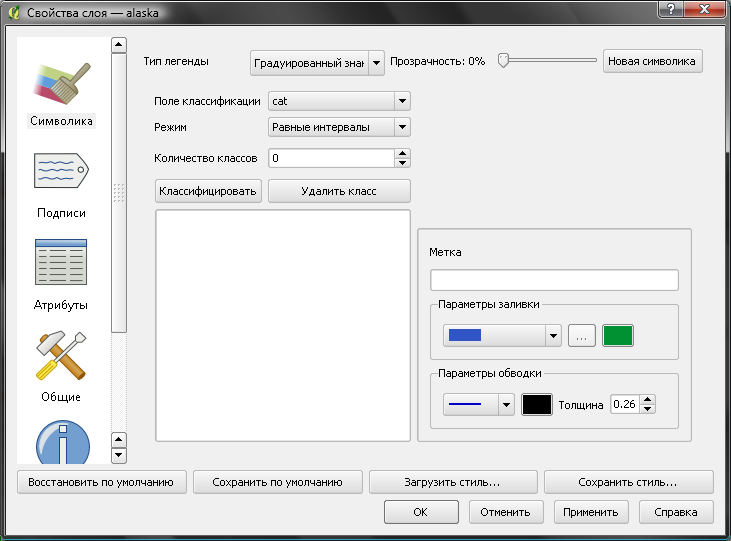
\includegraphics[clip=true, width=0.4\textwidth]{vectorClassifyGraduated}}\\
  \subfigure[Symbole gradu\'e] {\label{subfig:graduated_symbol}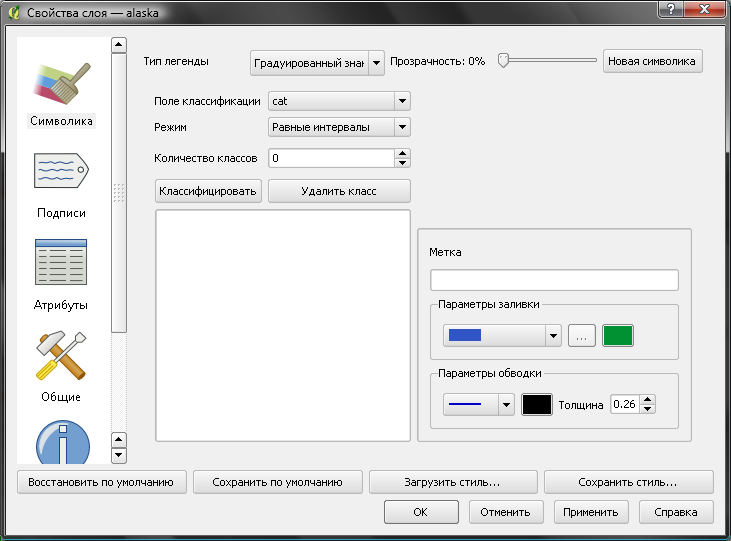
\includegraphics[clip=true, width=0.4\textwidth]{vectorClassifyGraduated}}\\
  %\subfigure[Continous color] {\label{subfig:cont_color}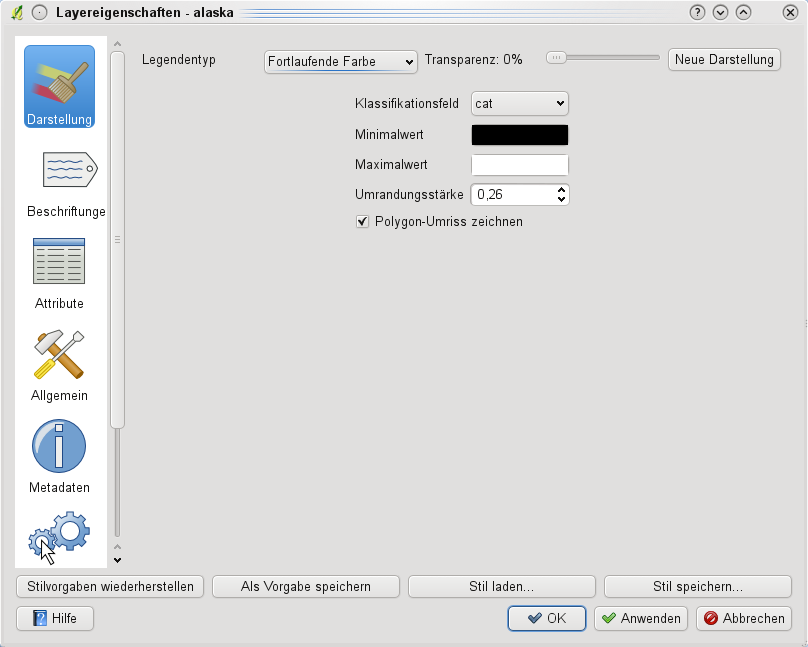
\includegraphics[clip=true, width=0.4\textwidth]{vectorClassifyContinous}}\goodgap
  \subfigure[Couleur continue] {\label{subfig:cont_color}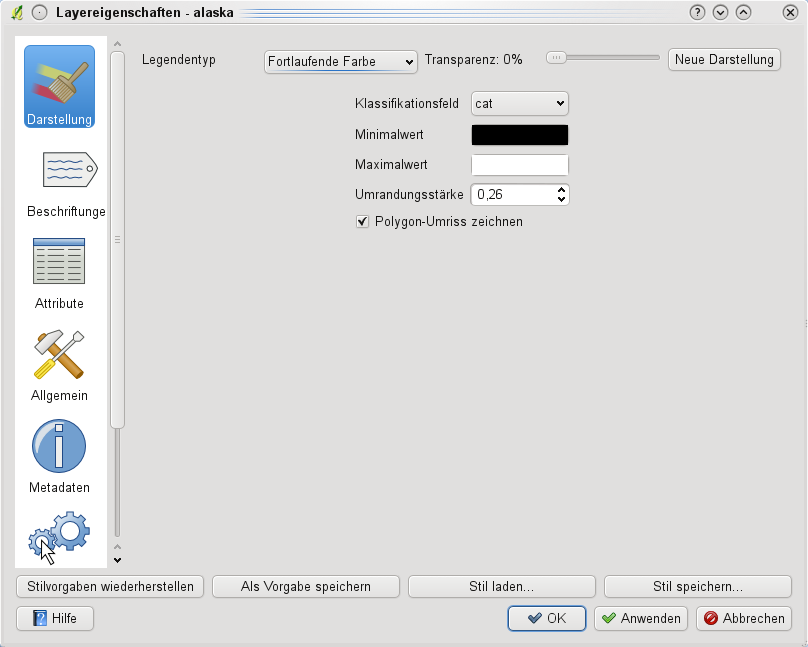
\includegraphics[clip=true, width=0.4\textwidth]{vectorClassifyContinous}}\goodgap
  %\subfigure[Unique value] {\label{subfig:unique_val}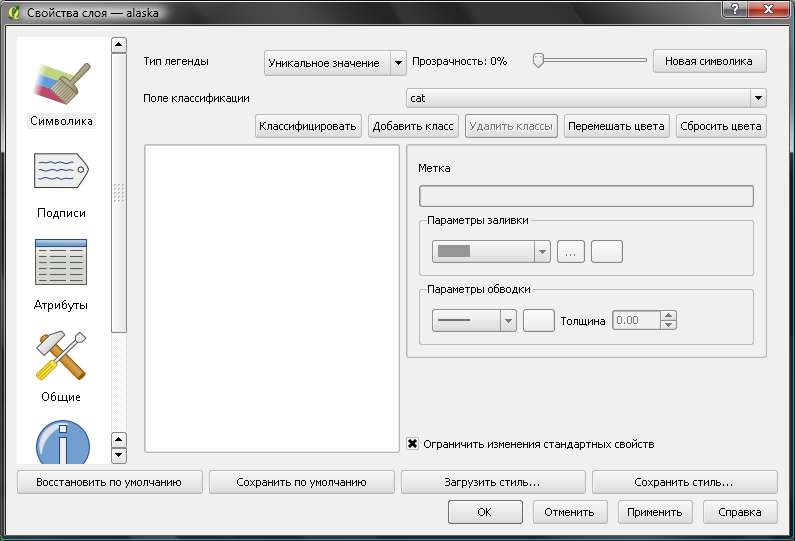
\includegraphics[clip=true, width=0.4\textwidth]{vectorClassifyUnique}}
  \subfigure[Valeur unique] {\label{subfig:unique_val}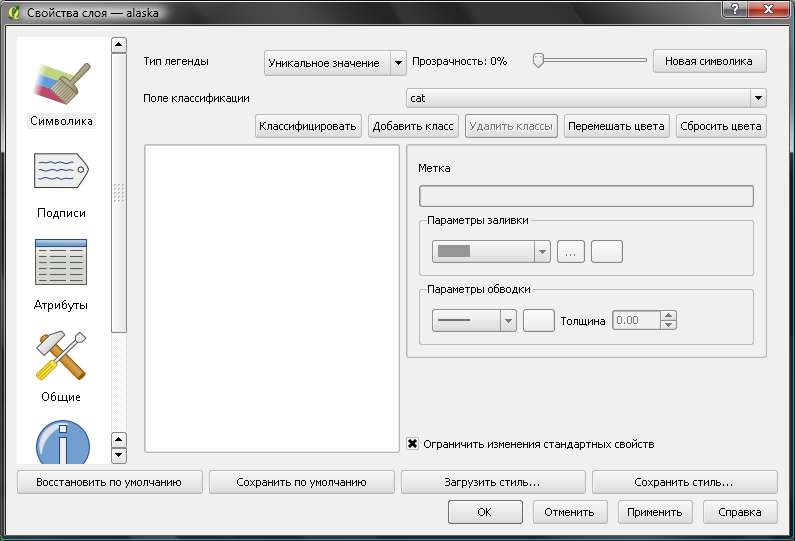
\includegraphics[clip=true, width=0.4\textwidth]{vectorClassifyUnique}}
\end{figure}

% FIXME: outdated
% Since \usertext{version v0.9} there is a function to use image files stored on
% your computer as fill pattern for vector layers.

%\minisec{Style Options} \label{sec:style_options} \index{vector layers!styles}
\minisec{Options de style} \label{sec:style_options}\index{couches vecteur!styles}
%Within this dialog you can style your vector layer. Depending on the selected rendering option you have the possibility to also classify your mapfeatures.
Dans cette fen\^etre vous pouvez donner un style \`a votre couche vecteur. Selon l'option de rendu s\'electionn\'ee, vous avez la possibilit\'e de classer vos entit\'es.

%At least the following styling options apply for nearly all renderers:
Les options de style suivantes s'appliquent quasiment \`a tous les types de rendus :
\begin{description}
%\item[Outline style] - pen-style for your outline of your feature. you can also set this to 'no pen'.
\item[Style du contour] - style de la ligne qui fait le contour de vos entit\'es. Vous pouvez \'egalement le d\'efinir \`a ``no pen'', pas de contour.
%\item[Outline color] - color of the ouline of your feature
\item[Couleur du contour] - couleur du contour de vos entit\'es.
%\item[Outline width] - width of your features
\item[\'Epaisseur du contour] - \'epaisseur du contour de vos entit\'es.
%\item[Fill color] - fill-color of your features.
\item[Couleur de remplissage] - couleur de remplissage de vos entit\'es.
%\item[Fill style] - Style for filling. Beside the given brushes you can select \selectstring{Fill style}{? texture} and click the \browsebutton button for selecting your own fill-style. Currently the fileformats \filename{*.jpeg, *.xpm, and *.png} are supported.
\item[Style de remplissage] - Style pour le remplissage. En plus des pinceaux propos\'es, vous pouvez s\'electionner \selectstring{Fill style}{? texture} et cliquez sur le \browsebutton bouton pour s\'electionner votre propre style de remplissage. Actuellement, les formats de fichier \filename{*.jpeg, *.xpm et *.png}.
\end{description}

%Once you have styled your layer you also could save your layer-style to a separate file (with \filename{*.qml}-ending). To do this, use the button \button{Save Style \ldots}. No need to say that \button{Load Style \ldots} loads your saved layer-style-file.
Une fois que vous avez d\'efini le style de votre couche, vous pouvez le sauvegarder dans un fichier s\'epar\'e (avec l'extension \filename{*.qml}). Pour faire cela, utilisez le bouton \button{Sauvegarder le style \ldots}. Inutile de dire que \button{Charger le style \ldots} charge vos fichiers sauvegard\'es.

%If you wish to always use a particular style whenever the layer is loaded, use the \button{Save As Default} button to make your style the default. Also, if you make changes to the style that you are not happy with, use the \button{Restore Default Styel} button to revert to your default style.
Si vous voulez utiliser en permanence un style particulier chaque fois que la couche est charg\'ee, utilisez le bouton \button{Sauvegarder comme d\'efaut} pour en faire le style par d\'efaut. Aussi, si le style ne vous plait pas et que vous le modifiez, utilisez le bouton \button{Restaurer le style par d\'efaut} pour en faire votre style par d\'efaut.

%\minisec{Vector transparency} \label{sec:vect_transparency} \index{vector layers!transparency}
\minisec{Transparence d'une couche vecteur} \label{sec:vect_transparency} \index{couches vecteur!transparence}
%QGIS \CURRENT allows to set a transparency for every vector layer. This can be done with the slider \slider{Transparency}{0}{20mm} inside the \tab{symbology} tab (see fig. \ref{fig:vector_symbology}). This is very useful for overlaying several vector layers.
QGIS \CURRENT permet de d\'efinir une transparence pour chaque couche vecteur. Ceci peut-\^etre fait avec le curseur \slider{Transparence}{0}{20mm} de l'onglet \tab{Convention des signes} (voir fig. \ref{fig:vector_symbology}). Ceci est tr\`es utile pour superposer plusieurs couches vecteur.

%\subsubsection{Metadata Tab}
\subsubsection{Onglet M\'etadadonn\'ees}

%The \tab{Metadata} tab contains information about the layer, including specifics about the type and location, number of features, feature type, and the editing capabilities. The \guiheading{Layer Spatial Reference System} section, providing projection information, and the \guiheading{Attribute field info} section, listing fields and their data types, are displayed on this tab. This is a quick way to get information about the layer.
L'onglet \tab{M\'etadadonn\'ees} contient les informations sur la couche dont le type et la localisation, le nombre d'entit\'es, le type des entit\'es et les possibilit\'es d'\'editions. Les sections \guiheading{Syst\`eme spatial de r\'ef\'erence de la couche} qui fournit les informations sur la projection et \guiheading{Information de champ d'attribut} qui liste les champs et leur type sont affich\'ees dans cet onglet. Cet onglet constitue un moyen rapide d'obtenir des informations sur une couche.

%\subsubsection{Labels Tab}
\subsubsection{Onglet \'Etiquettes}

%The \tab{Labels} tab allows you to enable labeling features and control a number of options related to fonts, placement, style, alignment and buffering.
L'onglet \tab{\'Etiquettes} vous permet d'activer la fonctionnalit\'e d'\'etiquetage et de g\'erer un certain nombre d'options li\'ees \`a la police de caract\`ere, au placement, au style, \`a l'alignement et au buffering.

%We will illustrate this by labelling the lakes shapefile of the \filename{qgis\_example\_dataset}:
Nous allons illustrer tout cela en \'etiquetant le shapefile des lacs du jeu de donn\'ees \filename{qgis\_example\_dataset} :

\begin{enumerate}
%\item Load the Shapefile \filename{alaska.shp} and GML file \filename{lakes.gml} in QGIS.
\item Charger le shapefile \filename{alaska.shp} et le fichier GML \filename{lakes.gml} dans QGIS.
%\item Zoom in a bit to your favorite area with some lake.
\item Zoommez l\'eg\`erement sur votre coin pr\'ef\'er\'e avec quelques lacs.
%\item Make the \filename{lakes} layer active.
\item Rendez active la couche \filename{lakes}
%\item Open the \dialog{Layer Properties} dialog.
\item Ouvrez la fen\^etre \dialog{Propri\'et\'es de la couche}.
%\item Click on the \tab{Labels} tab.
\item Cliquez sur l'onglet \tab{\'Etiquettes}.
%\item Check the \checkbox{Display labels} checkbox to enable labeling.
\item Cochez la case \checkbox{Afficher les \'etiquettes} pour activer l'\'etiquetage.
%\item Choose the field to label with. We'll use \selectstring{Field containing label}{NAMES}.
\item Choisissez le champ \`a utiliser pour les \'etiquettes. Ici, nous utiliserons le \selectstring{Field containing label}{NAMES}.
%\item Enter a default for lakes that have no name. The default label will be used each time QGIS encounters a lake with no value in the \guilabel{NAMES} field.
\item Choisissez un libell\'e par d\'efaut pour les lacs n'ayant pas de nom. Ce libell\'e sera utilis\'e chaque fois que QGIS rencontre un lac n'ayant pas de valeur dans le champ \guilabel{NAMES}.
%\item Click \button{Apply}.
\item Cliquez sur \button{Appliquer}.
\end{enumerate}

%Now we have labels. How do they look? They are probably too big and poorly placed in relation to the marker symbol for the lakes.
Maintenant, nous avons des \'etiquettes. De quoi ont-elles l'air ? Elles sont probablement trop grandes et mal plac\'ees par rapport au symbole marqueur des lacs.

%Select the \tab{Font} entry and use the \button{Font} and \button{Color} buttons to set the font and color. You can also change the angle and the placement of the text-label.
S\'electionnez l'entr\'ee \tab{Police} et utilisez les boutons \button{Police} et \button{Couleur} pour d\'efinir la police et la couleur. Vous pouvez \'egalement changer l'angle et le placement de l'\'etiquette.

%To change the position of the text relative to the feature:
Pour changer la position du texte par rapport \`a l'entit\'e :

\begin{enumerate}
%\item Click on the \tab{Font} entry.
\item Cliquez sur l'entr\'ee \tab{Police}
%\item Change the placement by selecting one of the radio buttons in the \classname{Placement} group. To fix our labels, choose the \radiobuttonon{Right} radio button.
\item Changer le placement en s\'electionnant l'un des boutons radio dans le groupe \classname{Placement}. Pour corriger nos \'etiquettes, choisissez le bouton radio \radiobuttonon{Droite}.
%\item the \classname{Font size units} allows you to select between \radiobuttonon{Points} or \radiobuttonon{Map units}.
\item La \classname{Taille de la police des unit\'es} vous permet de choisir entre  des \radiobuttonon{Points} ou des \radiobuttonon{Unit\'es de carte}
%\item Click \button{Apply} to see your changes without closing the dialog.
\item Cliquez sur \button{Appliquer} pour visualiser les changements sans fermer la fen\^etre.
\end{enumerate}

%Things are looking better, but the labels are still too close to the marker. To fix this we can use the options on the \tab{Position} entry. Here we can add offsets for the X and Y directions. Adding an X offset of 5 will move our labels off the marker and make them more readable. Of course if your marker symbol or font is larger, more of an offset will be required.
Ca \`a l'air plus joli mais les \'etiquettes sont encore trop proches des marqueurs. Pour corriger cela, nous pouvons utiliser les options de l'entr\'ee \tab{Position}. Ici, nous pouvons ajouter un d\'ecalage dans les directions X et Y. Ajouter un d\'ecalage de 5 en X d\'eplacera vos \'etiquettes et les rendra plus lisibles. Bien s\^ur si vos symboles marqueurs ou votre police sont plus grands un d\'ecalage plus important sera n\'ecessaire.

%The last adjustment we'll make is to \tab{buffer} the labels. This just means putting a backdrop around them to make them stand out better. To buffer the lakes labels:
Un dernier ajustement reste \`a faire sur les \'etiquettes : un \tab{buffer}. Il s'agit de cr\'eer un fond autour des \'etiquettes pour les faire mieux ressortir. Pour faire un buffer sur les \'etiquettes des lacs :

\begin{enumerate}
%\item Click the \tab{Buffer} tab.
\item Cliquez sur l'entr\'ee \tab{Buffer}.
%\item Click the \checkbox{Buffer Labels?} checkbox to enable buffering.
\item Cliquez sur la case \`a cocher \checkbox{Buffer Labels?} pour activer le buffer.
%\item Choose a size for the buffer using the spin box.
\item Choisissez une taille de buffer en utilisant les fl\`eches.
%\item Choose a color by clicking on \button{Color} and choosing your favorite from the color selector. You can also set some transparency for the  buffer if you prefer.
\item Choisissez une couleur en cliquant sur \button{Couleur} puis choisissez votre couleur favorite gr\^ace au s\'electeur. Si vous le souhaitez, vous pouvez \'egalement ajouter un peu de transparence au buffer.
%\item Click \button{Apply} to see if you like the changes.
\item Cliquez sur \button{Appliquer} pour voir si les changements vous plaisent.
\end{enumerate}

%If you aren't happy with the results, tweak the settings and then test again by clicking \button{Apply}.
Si le r\'esultat ne vous pla\^it pas, ajustez les param\`etres et re-testez en cliquant sur \button{Appliquer}.

%A buffer of 1 points seems to give a good result. Notice you can also specify the buffer size in map units if that works out better for you.
Un buffer d'un point semble donner un bon r\'esultat. Notez que vous pouvez \'egalement sp\'ecifier une taille de buffer en unit\'es de la carte si cela vous convient mieux.

%The remaining entries inside the \tab{Label} tab allow you control the appearance of the labels using attributes stored in the layer. The entries beginning with \tab{Data defined} allow you to set all the parameters for the labels using fields in the layer.
Les autres entr\'ees de l'onglet \tab{\'Etiquettes} vous permettent de contr\^oler l'apparence des \'etiquettes en utilisant les attributs stock\'es dans la couche. Les entr\'ees commen\c{c}ant par \tab{Data defined} vous permettent de d\'efinir tous les param\`etres des \'etiquettes en utilisant des champs de la couche.

%Not that the \tab{Label} tab provides a \classname{preview-box} where your selected label is shown.
Notez que l'onglet \tab{\'Etiquettes} propose une \classname{Pr\'evisualisation} montrant une de vos \'etiquettes.

%\subsubsection{Actions Tab}\index{actions}\label{label_actions}
\subsubsection{Onglet Actions}\index{actions}\label{label_actions}

%QGIS provides the ability to perform an action based on the attributes of a feature. This can be used to perform any number of actions, for example, running a program with arguments built from the attributes of a feature or passing parameters to a web reporting tool.
QGIS est capable d'effectuer des actions bas\'ees sur les attributs d'une entit\'e. Il peut s'agir de nombreuses actions, par exemple ex\'ecuter un programme avec des arguments construits \`a partir des attributs d'une entit\'e, ou encore, passer des param\`etres \`a un outil de publication de rapports sur internet.

%Actions are useful when you frequently want to run an external application or view a web page based on one or more values in your vector layer. An example is performing a search based on an attribute value. This concept is used in the following discussion.
Les actions sont utiles si vous voulez ex\'ecuter fr\'equemment une application externe ou charger une page web bas\'ee sur une ou plusieurs valeurs de votre couche vecteur. Un exemple d'application serait d'effectuer une recherche bas\'ee sur une valeur d'attribut. C'est l'id\'ee utilis\'ee dans les paragraphes qui suivent.

%\minisec{Defining Actions}\index{actions!defining}
\minisec{D\'efinir des actions}\index{actions!d\'efinir}

%Attribute actions are defined from the vector \dialog{Layer Properties} dialog. To define an action, open the vector \dialog{Layer Properties} dialog and click on the \tab{Actions} tab. Provide a descriptive name for the action. The action itself must contain the name of the application that will be executed when the action is invoked. You can add one or more attribute field values as arguments to the application. When the action is invoked any set of characters that start with a \% followed by the name of a field will be replaced by the value of that field. The special characters \%\% \index{\%\%}will be replaced by the value of the field that was selected from the identify results or attribute table (see Using Actions below).  Double quote marks can be used to group text into a single argument to the program, script or command. Double quotes will be ignored if preceded by a backslash.
Les actions sur les attributs sont d\'efinies dans la fen\^etre \dialog{Propri\'et\'es de la couche} des couches vecteur. Pour d\'efinir une action, ouvrez la fen\^etre de \dialog{Propri\'et\'es de la couche} et cliquez sur l'onglet \tab{Actions}. Donnez un nom descriptif \`a l'action. L'action elle-m\^eme doit contenir le nom de l'application qui sera ex\'ecut\'ee quand l'action sera invoqu\'ee. Vous pouvez ajouter un ou plusieurs champs d'attributs comme argument pour l'application. Quand l'action est invoqu\'ee n'importe quelle cha\^ine de caract\`ere pr\'ec\'ed\'ee de \% et correspondant au nom d'un champ sera remplac\'e par la valeur de ce champ. Le caract\`ere sp\'ecial \%\% \index{\%\%} sera remplac\'e par la valeur d'un champ qui a \'et\'e s\'electionn\'e par le r\'esultat d'un Identifier ou dans la table d'attributs (voir Utiliser les actions, ci-dessous). Des guillemets peuvent \^etre utilis\'es pour grouper du texte en un seul argument pour le programme, le script ou la commande. Les guillemets seront ignor\'es s'ils sont pr\'ec\'ed\'es d'un antislash.

%If you have field names that are substrings of other field names (e.g., \usertext{col1} and \usertext{col10}) you should indicate so, by surrounding the field name (and the \% character) with square brackets (e.g., \usertext{[\%col10]}). This will prevent the \usertext{\%col10} field name being mistaken for the \usertext{\%col1} field name with a \usertext{0} on the end. The brackets will be removed by QGIS when it substitutes in the value of the field. If you want the substituted field to be surrounded by square brackets, use a second set like this: \usertext{[[\%col10]]}.
Si vous avez des noms de champs qui sont contenus dans d'autres noms de champs (par exemple, \usertext{col1} et \usertext{col10}), vous devez l'indiquer en entourant le nom de champ (le caract\`ere \%) par des crochets (par exemple \usertext{[\%col10]}). Ceci \'evitera de prendre le nom de champ \usertext{\%col10} pour \usertext{\%col1} avec un \usertext{0} \`a la fin. Les crochets seront retir\'es quand QGIS substituera le nom par la valeur du champ. Si vous voulez que le champ \`a substituer soit entour\'e de crochets, utilisez un deuxi\`eme jeu de crochets comme ici : \usertext{[[\%col10]]}.

%The \dialog{Identify Results} dialog box includes a {\em (Derived)} item that contains information relevant to the layer type. The values in this item can be accessed in a similar way to the other fields by using preceeding the derived field name by \usertext{(Derived).}. For example, a point layer has an \usertext{X} and \usertext{Y} field and the value of these can be used in the action with \usertext{\%(Derived).X} and \usertext{\%(Derived).Y}. The derived attributes are only available from the \dialog{Identify Results} dialog box, not the \dialog{Attribute Table} dialog box.
La fen\^etre \dialog{R\'esultats identifi\'es} inclue une entr\'ee {\em (D\'eriv\'e)} qui contient des informations pertinentes selon le type de couche. Les valeurs de cette entr\'ee sont accessibles de la m\^eme mani\`ere que les autres champs en ajoutant \usertext{(Derived).} avant le nom du champ. Par exemple, une couche de points \`a un champ \usertext{X} et \usertext{Y} et leur valeur peut \^etre utilis\'ee dans l'action avec \usertext{\%(Derived).X} et \usertext{\%(Derived).Y}. Les attributs d\'eriv\'es sont disponibles uniquement depuis la fen\^etre \dialog{R\'esultats identifi\'es} et pas la \dialog{Table d'attributs}.

%Two example actions are shown below:\index{actions!examples}
Deux exemples d'action sont propos\'es ci-dessous : \index{actions!exemples}

\begin{itemize}
  \item \usertext{konqueror http://www.google.com/search?q=\%nam}
  \item \usertext{konqueror http://www.google.com/search?q=\%\%}
\end{itemize}

%In the first example, the web browser konqueror is invoked and passed a URL to open. The URL performs a Google search on the value of the \usertext{nam} field from our vector layer. Note that the application or script called by the action must be in the path or you must provided the full path. To be sure, we could rewrite the first example as: \usertext{/opt/kde3/bin/konqueror http://www.google.com/search?q=\%nam}. This will ensure that the konqueror application will be executed when the action is invoked.
Dans le premier exemple, le navigateur internet konqueror est lanc\'e avec une URL. L'URL effectue une recherche Google sur la valeur du champ \usertext{nam} de la couche vecteur. Notez que l'application ou le script appel\'e par l'action doit \^etre dans le path sinon vous devez fournir le chemin complet vers l'application. Pour \^etre certain, nous pouvons r\'e\'ecrire le premier exemple de cette mani\`ere : \usertext{/opt/kde3/bin/konqueror http://www.google.com/search?q=\%nam}. Ceci assurera que l'application konqueror sera ex\'ecut\'ee quand l'action sera invoqu\'ee.

%The second example uses the \%\% notation which does not rely on a particular field for its value. When the action is invoked, the \%\% will be replaced by the value of the selected field in the identify results or attribute table.
Le deuxi\`eme exemple utilise la notation \%\% dont la valeur ne d\'epend pas d'un champ en particulier. Quand l'action est invoqu\'ee, \%\% sera remplac\'e par la valeur du champ s\'electionn\'e dans les r\'esultats de l'identification ou dans la table d'attributs.

%\minisec{Using Actions}\index{actions!using}\label{label_usingactions}
\minisec{Utiliser les actions}\index{actions!utiliser}\label{label_usingactions}
%Actions can be invoked from either the \dialog{Identify Results} dialog or an \dialog{Attribute Table} dialog. (Recall that these dialogs can be opened by clicking \toolbtntwo{mActionOpenTable}{Identify Features} or \toolbtntwo{mActionOpenTable}{Open Table}.)
Les actions peuvent \^etre invoqu\'ees soit depuis la fen\^etre \dialog{R\'esultats identifi\'es} soit depuis la \dialog{Table d'attributs}. (Rappelez-vous que ces fen\^etres s'ouvrent en cliquant sur \toolbtntwo{mActionOpenTable}{Identifier les donn\'ees} ou \toolbtntwo{mActionOpenTable}{Ouvrir la table d'attributs}.)
%To invoke an action, right click on the record and choose the action from the popup menu. Actions are listed in the popup menu by the name you assigned when defining the actions. Click on the action you wish to invoke.
Pour invoquer une action, faites un clic-droit sur un enregistrement et choisissez l'action depuis le menu qui appara\^it. Les actions sont list\'ees dans le menu par le nom que vous leur avez donn\'e en les d\'efinissant. Cliquez ensuite sur l'action que vous souhaitez invoquer.

%If you are invoking an action that uses the \%\% notation, right-click on the field value in the \dialog{Identify Results} dialog or the \dialog{Attribute Table} dialog that you wish to pass to the application or script.
Si vous invoquez une action qui utilise la notation \%\%, faites un clic droit sur la valeur du champ que vous souhaitez passer en argument \`a l'application ou au script dans la fen\^etre \dialog{R\'esultats identifi\'es} ou la \dialog{Table d'attributs}.

%Here is another example that pulls data out of a vector layer and inserts them into a file using bash and the \usertext{echo} command (so it will only work \nix or perhaps \osx). The layer in question has fields for a species name \usertext{taxon\_name}, latitude \usertext{lat} and longitude \usertext{long}. I would like to be able to make a spatial selection of a localities and export these field values to a text file for the selected record (shown in yellow in the QGIS map area). Here is the action to achieve this:
Voici un autre exemple qui r\'ecup\`ere des donn\'ees d'une couche vecteur et qui les ins\`ere dans un fichier utilisant bash et la commande \usertext{echo} (cela ne marchera que sur \nix et peut-\^etre \osx). La couche en question \`a des champs pour le nom d'esp\`ece \usertext{taxon\_name}, la latitude \usertext{lat} et la longitude \usertext{long}. Je souhaiterais faire une s\'election spatiale des localit\'es et exporter ces valeurs des enregistrements s\'electionn\'es dans un fichier texte (ils apparaissent en jaune sur la carte dans QGIS). Voici l'action qui permettra de le faire :

\begin{verbatim}
  bash -c "echo \"%taxon_name %lat %long\" >> /tmp/species_localities.txt"
\end{verbatim}

%After selecting a few localities and running the action on each one, opening the output file will show something like this:
Apr\`es avoir s\'electionn\'e quelques localit\'es et lanc\'e l'action sur chacune, le fichier de destination ressemblera \`a \c{c}a :

\begin{verbatim}
  Acacia mearnsii -34.0800000000 150.0800000000
  Acacia mearnsii -34.9000000000 150.1200000000
  Acacia mearnsii -35.2200000000 149.9300000000
  Acacia mearnsii -32.2700000000 150.4100000000
\end{verbatim}

%As an exercise we create an action that does a Google search on the \filename{lakes} layer. First we need to determine the URL needed to perform a search on a keyword. This is easily done by just going to Google and doing a simple search, then grabbing the URL from the address bar in your browser. From this little effort we see that the format is: \url{http://google.com/search?q=qgis}, where \usertext{qgis} is the search term. Armed with this information, we can proceed:
Comme exercice, nous allons cr\'eer une action qui r\'ealise une recherche Google sur la couche \filename{lakes}. Tout d'abord, nous avons besoin de d\'eterminer l'URL n\'ecessaire pour effectuer une recherche sur un mot cl\'e. Il suffit simplement d'aller sur Google et faire une recherche simple puis r\'ecup\'erer l'URL dans la barre d'adresse de votre navigateur. De cela, nous en d\'eduisons la formulation : \url{http://google.com/search?q=qgis}, o\`u \usertext{qgis} est le terme recherch\'e. \`A partir de tout cela, nous pouvons poursuivre :

\begin{enumerate}
%\item Make sure the \filename{lakes} layer is loaded.
\item Assurez-vous que la couche \filename{lakes} est charg\'ee.
%\item Open the \dialog{Layer Properties} dialog by double-clicking on the layer in the legend or right-click and choose \dropmenuopt{Properties} from the popup menu.
\item Ouvrez la fen\^etre \dialog{Propri\'et\'es de la couche} en double cliquant sur la couche dans la l\'egende ou en faisant un clic-droit et en choisissant \dropmenuopt{Propri\'et\'es} dans le menu qui appara\^it.
%\item Click on the \tab{Actions} tab.
\item Cliquez sur l'onglet \tab{Actions}.
%\item Enter a name for the action, for example \usertext{Google Search}.
\item Entrez un nom pour l'action, par exemple \usertext{Recherche Google}
%\item For the action, we need to provide the name of the external program to run. In this case, we can use Firefox. If the program is not in your path, you need to provide the full path.
\item Pour l'action, nous devons fournir le nom du programme externe \`a lancer. Dans ce cas, nous allons utiliser Firefox. Si le programme n'est pas dans votre path, vous devez fournir le chemin complet.
%\item Following the name of the external application, add the URL used for doing a Google search, up to but not included the search term:  \url{http://google.com/search?q=}
\item A la suite du nom de l'application externe, ajoutez l'URL utilis\'ee pour faire la recherche Google, jusqu'au terme de recherche mais sans l'ajouter : \url{http://google.com/search?q=}
%\item The text in the \guilabel{Action} field should now look like this:\\
%\usertext{firefox \url{http://google.com/search?q=}}
\item Le texte dans le champ \guilabel{Action} devrait ressembler \`a \c{c}a :\\
\usertext{firefox \url{http://google.com/search?q=}}
%\item Click on the drop-down box containing the field names for the \usertext{lakes} layer. It's located just to the left of the \button{Insert Field} button.
\item Cliquez sur le menu d\'eroulant contenant les noms des champs pour la couche \usertext{lakes}. Il est situ\'e juste \`a gauche du bouton \button{Ins\'erer un champ}.
%\item From the drop-down box, select \selectstring{}{NAMES} and click \button{Insert Field}.
\item Dans le menu d\'eroulant, s\'electionnez \selectstring{}{NAMES} et cliquez sur \button{Ins\'erer un champ}.
%\item Your action text now looks like this:\\
%\usertext{firefox \url{http://google.com/search?q=\%NAMES}}
\item Le texte de votre action devrait maintenant ressembler \`a \c{c}a :\\
\usertext{firefox \url{http://google.com/search?q=\%NAMES}}
%\item Fo finalize the action click the \button{Insert action} button..
\item Pour finaliser l'action, cliquez sur le bouton \button{Ins\'erer une action}...
\end{enumerate}

%This completes the action and it is ready to use. The final text of the action should look like this:
L'action est donc enti\`erement d\'efinie et pr\^ete \`a \^etre utilis\'ee. Le texte final de l'action devrait correspondre \`a \c{c}a :

\begin{center}
\usertext{firefox \url{http://google.com/search?q=\%NAMES}}
\end{center}

%We can now use the action. Close the \dialog{Layer Properties} dialog and zoom in to an area of interest. Make sure the \filename{lakes} layer is active and identify a lake. In the result box you'll now see that our action is visible:
Nous pouvons maintenant utiliser l'action. Fermer la fen\^etre \dialog{Propri\'et\'es de la couche} et zoomez sur une zone d'int\'er\^et. Assurez-vous que la couche \filename{lakes} est active puis identifiez un lac. Dans la fen\^etre de r\'esultats, vous constatez que notre action est maintenant visible :

\begin{figure}[H]
  \begin{center}
  %\caption{Select feature and choose action \nixcaption}\label{fig:identify_action}\smallskip
  \caption{S\'electionnez une entit\'e et choisissez une action \nixcaption}\label{fig:identify_action}\smallskip
  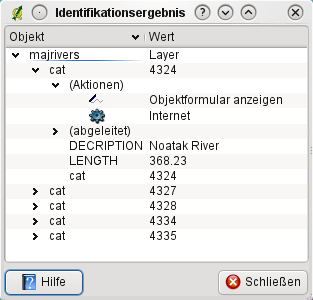
\includegraphics[clip=true, width=8cm]{action_identifyaction}
\end{center}
\end{figure}

%When we click on the action, it brings up Firefox and navigates to the URL \url{http://www.google.com/search?q=Tustumena}. It is also possible to add further attribute fields to the action. Therefore you can add a ``+'' to the end of the action text, select another field and click on \button{Insert Field}. In this example there is just no other field available that would make sense to search for.
Quand vous cliquez sur l'action, cela ouvre Firefox et charge l'URL \url{http://www.google.com/search?q=Tustumena}. Il est \'egalement possible d'ajouter d'autres champs attributs \`a l'action. Pour faire cela, vous pouvez ajouter un ``+'' \`a la fin du texte de l'action, s\'electionnez un autre champ et cliquez sur \button{Ins\'erer un champ}. Dans cet exemple, la recherche sur un autre champ n'aurait pas de sens.

%You can define multiple actions for a layer and each will show up in the \dialog{Identify Results} dialog. You can also invoke actions from the attribute table by selecting a row and right-clicking, then choosing the action from the popup menu.
Vous pouvez d\'efinir de multiples actions pour une couche et chacune apparaitra dans la fen\^etre \dialog{R\'esultats identifi\'es}. Vous pouvez \'egalement invoquer des actions depuis la table d'attributs en s\'electionnant une colonne et en faisant un clic-droit puis en choisissant l'action dans le menu qui appara\^it.

%You can think of all kinds of uses for actions. For example, if you have a point layer containing locations of images or photos along with a file name, you could create an action to launch a viewer to display the image. You could also use actions to launch web-based reports for an attribute field or combination of fields, specifying them in the same way we did in our Google search example.
Vous pouvez imaginer toute sorte d'utilisations pour ces actions. Par exemple, si vous avait une couche de points contenant la localisation d'images ou de photos ainsi qu'un nom de fichier, vous pouvez cr\'eer une action qui lancera un visualisateur pour afficher les images. Vous pouvez \'egalement utiliser les actions pour lancer des rapports sur internet pour un champ attributaire ou une combinaison de champs, en les sp\'ecifiant de la m\^eme mani\`ere que pour une recherche

%\subsubsection{Attributes Tab}\index{attributes}\label{label_attributes}
\subsubsection{Onglet attributs}\index{attributs}\label{label_attributes}
%Within the \tab{Attributes} tab the attributes of the selected dataset can be manipulated. The buttons \button{New Column} and \button{Delete Column} can be used, when the dataset is in editing mode. At the moment only columns from PostGIS layers can be edited, because this feature is not yet supported by the OGR library.
Dans l'onglet \tab{Attributs}, il est possible de manipuler les attributs du jeu de donn\'ees s\'electionn\'e. Les boutons \button{Ajouter une colonne} et \button{Supprimer une colonne} peuvent \^etre utilis\'es lorsque le jeu de donn\'ees est en mode \'edition. A ce moment les colonnes des couches PostGIS seulement peuvent \^etre \'edit\'ees car cette fonctionnalit\'e n'est pas encore support\'ee dans la biblioth\`eque OGR.

%The \button{Toggle editing mode} button toggles this mode.
Le bouton \button{Basculer en mode \'edition} permet de passer dans ce mode.

%\minisec{edit widget}
\minisec{widget d'\'edition}

%Within the \tab{Attributes} tab you also find an \texttt{edit widget} and a \texttt{value} column. These two columns can be used to define values or a range of values that are allowed to be added to the specific attribute table columns. They are used to produce different edit widgets in the attribute dialog. These widgets are:
Dans l'onglet \tab{Attributs} vous trouverez un colonne \texttt{Editer le bidule} et une colonne \texttt{valeur}. Ces deux colonnes peuvent \^etre utilis\'ees pour d\'efinir les valeurs ou les plages de valeurs permises lors de l'ajout d'attributs dans une colonne. Elles sont utilis\'ees pour g\'en\'erer diff\'erents widgets d'\'edition dans la fen\^etre des attributs. Ces widgets sont :

\begin{itemize}
%\item line edit: an edit field which allows to enter simple text (or restrict to numbers for numeric attributes).
\item \'edition de ligne : un champ d'\'edition qui permet d'entrer du texte simple (ou de restreindre \`a des nombres pour des attributs de type num\'eriques).
%\item unique value: a list of unique attribute values of all pre-existing features is produced and presented in a combo box for selection.
\item valeurs uniques : une liste de valeurs d'attribut uniques de toutes les entit\'es pr\'e-existantes et pr\'esent\'ees dans la liste d\'eroulante pour s\'election.
%\item  unique value (editable): a combination of `line edit' and `unique value'. The edit field completes entered values to the unique value, but also allows to enter new values.
\item valeur unique (\'editable) : une combinaison de `\'edition de ligne' et `valeurs uniques'. Le champ \'edit\'e autorise les nouvelles valeurs et les ajoute \`a la liste des valeurs uniques.
%\item value map: a combobox to select from a set of values specified in the \texttt{value} column the \tab{Attributes} tab.  The possible values are delimited by a semicolon (e.g. \verb|high;medium;low|).  It is also possible to prepend a label to each value, which is delimited with an equal sign (e.g. \verb|high=1;medium=2;low=3|). The label is shown in the combobox instead of the value.
\item Palette de valeur : une liste d\'eroulante pour s\'electionner une valeur dans une liste sp\'ecifi\'ee dans le champ \texttt{valeurs} de l'onglet \tab{Attributs}. Les valeurs possibles sont d\'elimit\'ees par un point virgule (par exemple \verb|fort;moyen;faible|). Il est \'egalement possible d'associer une \'etiquette \`a chaque valeur, qui sera d\'elimit\'ee par un signe \'egal (par exemple \verb|fort=1;moyen=2;faible=3|). L'\'etiquette sera visible dans la liste d\'eroulante \`a la place de la valeur.
%\item classification: if a unique value renderer is selected for the layer, the values used for the classes are presented for selection in a combobox.
\item classification :  si un rendu de type valeur unique est choisi pour la couche, ces valeurs seront utilis\'ees pour les classes propos\'ees pour la s\'election dans la liste d\'eroulante.
%\item range (editable): A edit field that allows to restrict numeric values to a given range.  That range is specified by entering minium and maximum value delimited by a semicolon (e.g. \verb|0;360|) in the \texttt{value} column of the \tab{Attributes} tab.
\item Domaine de validit\'e (\'editable) : un champ d'\'edition qui permet de restreindre les valeurs num\'eriques \`a une plage donn\'ee. Cette plage est sp\'ecifi\'ee en entrant les valeurs minimum et un maximum d\'elimit\'ees par un point virgule (par exemple \verb|0;360|) dans le champ \texttt{valeurs} de l'onglet \tab{Attributs}.
%\item range (slider): A slider widget is presented that allows selection of a value in a given range and precision.  The range is specifed by minimum, maximum value and a step width (e.g. \verb|0;360;10|) in the \texttt{value} column of the \tab{Attributes} tab.
\item Domaine de validit\'e (barre de d\'efilement) : une barre de d\'efilement permet de s\'electionner une valeur dans une plage et avec une pr\'ecision donn\'ees. La plage est sp\'ecifi\'ee par des valeurs minimum et maximum et un pas (par exemple \verb|0;360;10|) dans le champ \texttt{valeurs} de l'onglet \tab{Attributs}.
%\item file name: the line edit widget is accompanied by a push button. When pressed it allows to select a filename using the standard file dialog.
\item nom de fichier : le widget d'\'edition de ligne est accompagn\'e d'un bouton. Press\'e, il permet de s\'electionner un nom de fichier gr\^ace \`a une fen\^etre standard d'exploration des fichiers.
\end{itemize}

%\subsection{Editing}\index{editing}
\subsection{\'Editer}\index{\'editer}

%QGIS supports basic capabilities for editing vector geometries.  Before reading any further you should note that at this stage editing support is still preliminary. Before performing any edits, always make a backup of the dataset you are about to edit.
Les capacit\'es d'\'edition de QGIS sur les g\'eom\'etries vecteur sont basiques. Avant d'aller plus loin, notez que la gestion de l'\'edition dans QGIS reste encore pr\'eliminaire. Avant d'effectuer des \'editions, cr\'eez toujours une sauvegarde du jeu de donn\'ees que vous allez \'editer.

%\textbf{Note} - the procedure for editing GRASS layers is different - see Section \ref{grass_digitising} for details.
\textbf{Note} - la proc\'edure pour \'editer des couches GRASS est diff\'erente - voir Section \ref{grass_digitising} pour plus de d\'etails.

%\subsubsection{Setting the Snapping Tolerance and Search Radius}
\subsubsection{D\'efinir le rayon de tol\'erance d'accrochage et de recherche}

%Before we can edit vertices, it is very important to set the snapping tolerance and search radius to a value that allows us an optimal editing of the vector layer geometries.
Avant de pouvoir \'editer des sommets, il est tr\`es important de fixer la tol\'erance d'accrochage et le rayon de recherche \`a des valeurs qui nous permettent d'\'editer les g\'eom\'etries vecteur de mani\`ere optimale.

%\minisec{Snapping tolerance}
\minisec{Tol\'erance d'accrochage}

%Snapping tolerance is the distance QGIS uses to \usertext{search} for the closest vertex and/or segment you are trying to connect when you set a new vertex or move an existing vertex. If you aren't within the snap tolerance, QGIS will leave the vertex where you release the mouse button, instead of snapping it to an existing vertex and/or segment.
La tol\'erance d'accrochage est la distance que QGIS utilise pour \usertext{chercher} le sommet ou le segment le plus pr\`es que vous cherchez \`a connecter lorsque vous cr\'eez un nouveau sommet ou en d\'eplacez un existant. Si vous n'\^etes pas dans la tol\'erance d'accrochage, QGIS va laisser le vertex \`a l'endroit o\`u vous l\^achez le bouton de la souris, au lieu de l'accrocher \`a un sommet ou un segment existant.

\begin{enumerate}
%\item A general, project wide snapping tolerance can be defined choosing \mainmenuopt{Settings} > \dropmenuopttwo{mActionOptions}{Options}. In the \tab{Digitizing} tab you can select between to vertex, to segment or to vertex and segment as default snap mode. You can also define a default snapping tolerance and a search radius for vertex edits. Remember the tolerance is in layer units. In our digitizing project (working with the Alaska dataset), the units are in feet. Your results may vary, but something on the order of 300ft should be fine at a scale of 1:10 000 should be a reasonable setting.
\item Une tol\'erance g\'en\'erale, commune \`a tout le projet, peut-\^etre d\'efinie dans \mainmenuopt{Pr\'ef\'erences} > \dropmenuopttwo{mActionOptions}{Options}. Dans l'onglet \tab{Num\'erisation}, vous pouvez choisir le mode d'accrochage par d\'efaut : sur un sommet, sur un segment ou sur un sommet ou un segment. Vous pouvez \'egalement d\'efinir une tol\'erance d'accrochage par d\'efaut et un rayon de recherche pour les \'editions de sommets. Rappelez-vous que la tol\'erance est dans l'unit\'e de la couche. Dans notre projet de num\'erisation (travail sur le jeu de donn\'ees Alaska), les unit\'es sont en pieds. Le r\'esultat peut varier mais une tol\'erance de l'ordre de 300 pieds devrait \^etre convenable \`a une \'echelle de 1:10 000.
%\item A layer based snapping tolerance can be defined by choosing \mainmenuopt{Settings} > \dropmenuopttwo{mActionOptions}{Project Properties\dots}. In the \tab{General} tab, section \classname{Digitize} you can click on \button{Snapping options\dots} to enable and adjust snapping mode and tolerance on a layer basis (see Figure~\ref{fig:snappingoptions}).
\item Une tol\'erance d'accrochage li\'ee \`a une couche peut \^etre d\'efinie dans \mainmenuopt{Pr\'ef\'erences} > \dropmenuopttwo{mActionOptions}{Propri\'et\'es du projet\dots}. Dans l'onglet \tab{G\'en\'eral}, section \classname{Num\'eriser}, vous pouvez cliquer sur \button{Options d'accrochage\dots} pour activer et ajuster le mode d'accrochage et la tol\'erance pour chaque couche  (voir Figure~\ref{fig:snappingoptions}).
\end{enumerate}

\begin{figure}[H]
  \begin{center}
  %\caption{Edit snapping options on a layer basis \nixcaption}\label{fig:snappingoptions}\smallskip
  \caption{\'Edition des options d'accrochage pour chaque couche \nixcaption}\label{fig:snappingoptions}\smallskip
  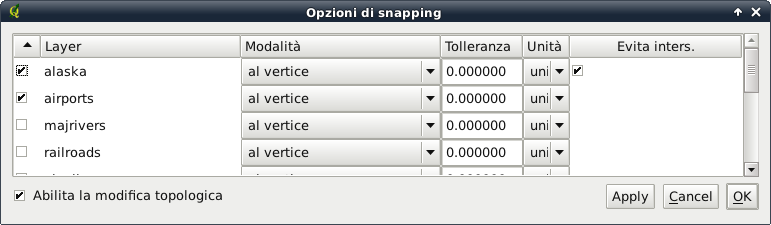
\includegraphics[clip=true, width=14cm]{editProjectSnapping}
\end{center}
\end{figure}

%\minisec{Search radius}
\minisec{Rayon de recherche}

%Search radius is the distance QGIS uses to \usertext{search} for the closest vertex you are trying to move when you click on the map. If you aren't within the search radius, QGIS won't find and select any vertex for editing and it will pop up an annoying warning to that effect. Snap tolerance and search radius are set in map units so you may find you need to experiment to get them set right. If you specify too big of a tolerance, QGIS may snap to the wrong vertex, especially if you are dealing with a large number of vertices in close proximity. Set search radius too small and it won't find anything to move.
Le rayon de recherche est la distance que QGIS utilise pour \usertext{chercher} le sommet le plus proche que vous souhaitez d\'eplacer quand vous cliquez sur la carte. Si vous n'\^etes pas dans le rayon de recherche, QGIS ne trouvera ni ne s\'electionnera de sommet \`a \'editer et une fen\^etre d'alerte d\'esagr\'eable apparaitra. La tol\'erance d'accrochage et le rayon de recherche sont d\'efinis dans les unit\'es de la carte, vous allez peut-\^etre avoir besoin d'exp\'erimenter diff\'erentes valeurs avant de trouver la bonne. Si vous sp\'ecifiez une tol\'erance trop grande, QGIS risque d'accrocher le mauvais sommet, surtout si vous avez un grand nombre de sommets \`a proximit\'e. D\'efinissez un rayon de recherche trop petit et QGIS ne trouvera rien \`a d\'eplacer.

%The search radius for vertex edits in layer units can be defined in the \tab{Digitizing} tab under \mainmenuopt{Settings} > \dropmenuopttwo{mActionOptions}{Options}. The same place where you define the general, project wide snapping tolerance.
Le rayon de recherche pour l'\'edition des sommets dans l'unit\'e de la couche peut \^etre d\'efini dans l'onglet \tab{Num\'erisation} de \mainmenuopt{Pr\'ef\'erences} > \dropmenuopttwo{mActionOptions}{Options}. Au m\^eme endroit que vous d\'efinissez la tol\'erance d'accrochage pour tout le projet.

%\subsubsection{Topological editing}
\subsubsection{\'Edition topologique}

%Besides layer based snapping options the \tab{General} tab in menu \mainmenuopt{Settings} -> \dropmenuopttwo{mActionOptions}{Project Properties\dots} also provides some topological functionalities. In the Digitizing option group you can \checkbox{Enable topological editing} and/or activate \checkbox{Avoid intersections of new polygons}.
En plus des options d'accrochage pour chaque couche, l'onglet \tab{G\'en\'eral} du menu \mainmenuopt{Pr\'ef\'erences} > \dropmenuopttwo{mActionOptions}{Propri\'et\'es du projet\dots} propose quelques fonctionnalit\'es topologiques. Dans le groupe d'options de Num\'erisation, vous pouvez \checkbox{Activer l'\'edition topologique} et/ou activer \checkbox{\'Eviter les intersections de nouveaux polygones}.

%\minisec{Enable topological editing}
\minisec{Activer l'\'edition topologique}

%The option \checkbox{Enable topological editing} is for editing and maintaining common boundaries in polygon mosaics. QGIS "detects" a shared boundary in a polygon mosaic and you only have to move the vertex once and QGIS will take care about updating the other boundary.
L'option \checkbox{Activer l'\'edition topologique} permet d'\'editer en gardant des limites communes entre les polygones. QGIS "d\'etecte" une limite commune entre les polygones et vous avez simplement \`a d\'eplacer le sommet une fois et QGIS s'occupera de mettre \`a jour l'autre limite.

%\minisec{Avoid intersections of new polygons}
\minisec{\'Eviter les intersections de nouveaux polygones}

%The second topological option called \checkbox{Avoid intersections of new polygons} avoids overlaps in polygon mosaics. It is for quicker digitizing of adjacent polygons. If you already have one polygon, it is possible with this option to digitise the second one such that both intersect and qgis then cuts the second polygon to the common boundary. The advantage is that users don't have to digitize all vertices of the common boundary.
La deuxi\`eme option topologique, \checkbox{\'Eviter les intersections de nouveaux polygones}, permet d'\'eviter des recouvrements entre les polygones. Cela permet de num\'eriser des polygones adjacents plus rapidement. Si vous avez d\'ej\`a un polygone, avec cette option, vous pouvez num\'eriser le second de mani\`ere \`a ce qu'ils intersectent et QGIS coupera le second polygone aux limites communes. L'avantage est que les utilisateurs n'ont pas \`a num\'eriser tous les sommets des limites communes.

%\subsubsection{Editing an Existing Layer}
\subsubsection{\'Edition d'une couche existante}
\index{couches vecteur!\'editer}
\index{editer!une couche existante}
\label{sec:edit_existing_layer}

%By default, QGIS loads layers read-only: This is a safeguard to avoid accidentally editing a layer if there is a slip of the mouse. However, you can choose to edit any layer as long as the data provider supports it, and the underlying data source is writable (i.e. its files are not read-only).
Par d\'efaut, QGIS charge les couches en lecture seule : c'est une s\'ecurit\'e pour \'eviter d'\'editer accidentellement une couche si la souris a gliss\'e. Cependant, vous pouvez choisir d'\'editer une couche du moment que le fournisseur de donn\'ees le g\`ere et que la source de donn\'ees est \'editable (i.e. fichiers qui ne sont pas en lecture seule).

%Layer editing is most versatile when used on PostgreSQL/PostGIS data sources.
L'\'edition d'une couche est plus flexible lorsqu'il s'agit de sources de donn\'ees PostgreSQL/PostGIS.

%\begin{Tip}[ht]\caption{\textsc{Data Integrity}}
\begin{Tip}[ht]\caption{\textsc{Int\'egrit\'e des donn\'ees}}
%\qgistip{It is always a good idea to back up your data source before you start editing. While the authors of QGIS have made every effort to preserve the integrity of your data, we offer no warranty in this regard.}
\qgistip{Sauvegarder vos donn\'ees avant de se lancer dans une \'edition est toujours une bonne id\'ee. Bien que les auteurs de QGIS ont fait beaucoup d'efforts pour pr\'eserver l'int\'egrit\'e de vos donn\'ees, nous n'offrons aucune garantie.}
\end{Tip}

%\begin{Tip}[ht]\caption{\textsc{Manipulating Attribute data}}
\begin{Tip}[ht]\caption{\textsc{Manipulation des donn\'ees attributaires}}
%\qgistip{Currently only PostGIS layers are supported for adding or dropping attribute columns within this dialog. In future versions of QGIS, other datasources will be supported, because this feature was recently implemented in GDAL/OGR > 1.6.0}
\qgistip{Actuellement, seules les couches PostGIS g\`erent l'ajout ou la suppression de champs attributaires dans cette fen\^etre. Dans les versions futures de QGIS, d'autres sources de donn\'ees seront g\'er\'ees puisque cette fonctionnalit\'e a r\'ecemment \'et\'e ajout\'ee \`a GDAL/OGR > 1.6.0}
\end{Tip}

%\begin{Tip}[ht]\caption{\textsc{Save Regularly}}
\begin{Tip}[ht]\caption{\textsc{Fr\'equence de sauvegarde}}
%\qgistip{Remember to toggle \toolbtntwo{mActionToggleEditing}{Toggle editing} off regularly. This allows you to save your recent changes, and also confirms that your data source can accept all your changes.}
\qgistip{N'oubliez pas de cliquer sur \toolbtntwo{mActionToggleEditing}{Basculer en mode \'edition} r\'eguli\`erement. Cela vous permet de sauvegarder les changements r\'ecents mais \'egalement de confirmer que votre source de donn\'ees accepte tous vos changements.}
\end{Tip}

%\begin{Tip}[ht]\caption{\textsc{Concurrent Edits}}
\begin{Tip}[ht]\caption{\textsc{\'Editions concurrentes}}
%\qgistip{This version of QGIS does not track if somebody else is editing a feature at the same time as you. The last person to save their edits wins.}
\qgistip{Cette version de QGIS ne regarde pas si quelqu'un d'autre est en train d'\'editer une entit\'e en m\^eme temps que vous. La derni\`ere personne \`a sauvegarder ses \'editions gagne.}
\end{Tip}

%\begin{Tip}[ht]\caption{\textsc{Zoom in Before Editing}}
\begin{Tip}[ht]\caption{\textsc{Zoomez avant d'\'editer}}
%\qgistip{Before editing a layer, you should zoom in to your area of interest. This avoids waiting while all the vertex markers are rendered across the entire layer.}
\qgistip{Avant d'\'editer une couche, vous devez zoomer sur votre zone d'int\'er\^et. Cela \'evite les temps d'attente lorsque les marqueurs de sommets s'affichent pour toute la couche.}
\end{Tip}

%\begin{Tip}[ht]\caption{\textsc{Vertex Markers}}.
\begin{Tip}[ht]\caption{\textsc{Marqueurs de sommet}}
%\qgistip{The current version of QGIS supports two kinds of vertex-markers - a semi-transparent circle or a cross. To change the marker style, choose \dropmenuopttwo{mActionOptions}{Options} from the \mainmenuopt{Settings} menu and click on the \tab{Digitizing} tab and select the appropriate entry.}
\qgistip{La version actuelle de QGIS g\`ere deux type de marqueurs de sommet : un cercle semi-transparent ou une croix. Pour changer le style du marqueur, aller dans \dropmenuopttwo{mActionOptions}{Options} du menu \mainmenuopt{Pr\'ef\'erences} et cliquez sur l'onglet \tab{Num\'erisation} puis s\'electionnez les param\`etres appropri\'es.}
\end{Tip}

%All editing sessions start by choosing the \dropmenuopttwo{mActionToggleEditing}{Toggle editing} option. This can be found in the context menu after right clicking on the legend entry for that layer.\index{Allow Editing} Alternately, you can use the \index{Toggle Editing} \toolbtntwo{mActionToggleEditing}{Toggle editing} button from the toolbar to start or stop the editing mode.\index{editing!icons} Once the layer is in edit mode, markers will appear at the vertices, and additional tool buttons on the editing toolbar will become available.
Toute session d'\'edition commence par un clic sur \dropmenuopttwo{mActionToggleEditing}{Basculer en mode \'edition}. Ceci se trouve dans le menu contextuel qui appara\^it apr\`es un clic-droit sur la couche dans la l\'egende.\index{Autoriser l'\'edition} Sinon, vous pouvez utiliser le bouton \index{Basculer en mode \'edition} \toolbtntwo{mActionToggleEditing}{Basculer en mode \'edition} de la barre d'outils pour lancer ou stopper l'\'edition. \index{\'editer!ic\^ones} Une fois la couche en mode \'edition, les marqueurs apparaissent sur les sommets et de nouveaux outils de la barre d'outil \'edition sont disponibles.

%\minisec{Zooming with the mouse wheel}
\minisec{Zoomer avec la molette de la souris}

%While digitizing you can use the mouse wheel to zoom in and out on the map Place the mouse cursor inside the map area and roll it forward (away from you) to zoom in and backwards (towards you) to zoom out. The mouse cursor position will be the center of the zoomed area of interest. You can customize the behavior of the mouse wheel zoom using the \tab{Map tools} tab under the \mainmenuopt{Settings} >\dropmenuopt{Options} menu.
Lorsque vous num\'erisez, vous pouvez utiliser la molette de la souris pour zoomer et d\'ezoomer sur la carte. Placez le curseur de la souris dans la zone de carte et faites rouler la molette vers l'avant (loin de vous) pour zoomer et vers l'arri\`ere (vers vous) pour d\'ezoomer. La position du curseur de la souris correspondra au centre du zoom. Vous pouvez param\'etrer le comportement de la molette de la souris en allant dans l'onglet \tab{Outils cartographiques} dans le menu \mainmenuopt{Pr\'ef\'erences} >\dropmenuopt{Options}.

%\minisec{Panning with the arrow keys}
\minisec{Se d\'eplacer avec les fl\`eches de direction}

%Panning the Map during digitizing is possible with the arrow keys. Place the mouse cursor inside the map area and click on the right arrow key to pan east, left arrow key to pan west, up arrow key to pan north and down arrow key to pan south.
Se d\'eplacer sur la carte pendant la num\'erisation est possible avec les fl\`eches de direction. Placez le curseur de la souris sur la zone de carte et cliquez sur la touche fl\`eche droite pour vous d\'eplacer vers l'est, la fl\`eche gauche pour aller vers l'ouest, la fl\`eche haut pour le nord et la fl\`eche bas pour le sud.

%You can also use the spacebar to temporarily cause mouse movements to pan then map. The PgUp and PgDown keys on your keyboard will cause the map display to zoom in or out without interrupting your digitising session.
Vous pouvez \'egalement utiliser la barre d'espacement pour activer temporairement le d\'eplacement sur la carte par les mouvements de la souris. Les touches PgUp et PgDown de votre clavier provoqueront le zoom ou le d\'e-zoom sans interrompre la session d'\'edition.

%You can perform the following editing functions:
Vous pouvez r\'ealiser les fonctions d'\'edition suivantes :

\begin{itemize}
%\item Add Features: \toolbtntwo{mActionCapturePoint}{Capture Point}, \toolbtntwo{mActionCaptureLine}{Capture Line} and \toolbtntwo{mActionCapturePolygon}{Capture Polygon}
\item Ajouter des entit\'es : \toolbtntwo{mActionCapturePoint}{Capturer le Point}, \toolbtntwo{mActionCaptureLine}{Capturer la Ligne} et \toolbtntwo{mActionCapturePolygon}{Capturer le Polygone}
%\item \toolbtntwo{mActionAddRing}{Add Ring}
\item \toolbtntwo{mActionAddRing}{Ajouter Anneau}
%\item \toolbtntwo{mActionAddIsland}{Add Island}
\item \toolbtntwo{mActionAddIsland}{Ajouter Ile}
%\item \toolbtntwo{mActionSplitFeatures}{Split Features}
\item \toolbtntwo{mActionSplitFeatures}{Couper Objet}
%\item \toolbtntwo{mActionMoveFeature}{Move Features}
\item \toolbtntwo{mActionMoveFeature}{D\'eplacer Objet}
%\item \toolbtntwo{mActionMoveVertex}{Move Vertex}
\item \toolbtntwo{mActionMoveVertex}{D\'eplacer le Sommet}
%\item \toolbtntwo{mActionAddVertex}{Add Vertex}
\item \toolbtntwo{mActionAddVertex}{Ajouter un Sommet}
%\item \toolbtntwo{mActionDeleteVertex}{Delete Vertex}
\item \toolbtntwo{mActionDeleteVertex}{Effacer un Sommet}
%\item \toolbtntwo{mActionDeleteSelected}{Delete Selected}
\item \toolbtntwo{mActionDeleteSelected}{Effacer la S\'election}
%\item \toolbtntwo{mActionEditCut}{Cut Features}
\item \toolbtntwo{mActionEditCut}{Couper Entit\'es}
%\item \toolbtntwo{mActionEditCopy}{Copy Features}
\item \toolbtntwo{mActionEditCopy}{Copier Entit\'es}
%\item \toolbtntwo{mActionEditPaste}{Paste Features}
\item \toolbtntwo{mActionEditPaste}{Coller Entit\'es}
\end{itemize}

%\minisec{Adding Features}
%\index{vector layers!adding!feature}
\minisec{Ajouter des entit\'es}
\index{couches vecteur!ajouter!entit\'es}

%Before you start adding features, use the \toolbtntwo{mActionPan}{pan} and \toolbtntwo{mActionZoomIn}{zoom-in}/\toolbtntwo{mActionZoomOut}{zoom-out} tools to first navigate to the area of interest.
Avant de commencer \`a ajouter des entit\'es, utiliser les outils \toolbtntwo{mActionPan}{Se d\'eplacer dans la carte} et \toolbtntwo{mActionZoomIn}{zoom +}/\toolbtntwo{mActionZoomOut}{zoom -} pour naviguer vers la zone d'inter\^et.

%Then you can use the \toolbtntwo{mActionCapturePoint}{Capture point}, \toolbtntwo{mActionCaptureLine}{Capture line} or \toolbtntwo{mActionCapturePolygon}{Capture polygon} icons on the toolbar to put the QGIS cursor into digitizing mode.
Ensuite vous pouvez utiliser \toolbtntwo{mActionCapturePoint}{Capturer le Point}, \toolbtntwo{mActionCaptureLine}{Capturer la Ligne} ou \toolbtntwo{mActionCapturePolygon}{Capturer le Polygone} dans la barre d'outils pour mettre le curseur de QGIS en mode num\'erisation.

%For each feature, you first digitize the geometry, then enter its attributes.
Pour chaque entit\'e, vous num\'erisez d'abord la g\'eom\'etrie puis entrez les attributs.

%To digitize the geometry, left-click on the map area to create the first point of your new feature.
Pour num\'eriser la g\'eom\'etrie, faites un clic-gauche sur la zone de la carte pour cr\'eer le premier point de votre nouvelle entit\'e.

%For lines and polygons, keep on left-clicking for each additional point you wish to capture.  When you have finished adding points, right-click anywhere on the map area to confirm you have finished entering the geometry of that feature.
Pour les lignes ou les polygones, continuer \`a faire des clics-gauche pour chaque nouveau point que vous souhaitez capturer. Lorsque vous avez fini d'ajouter des points, faites un clic-droit n'importe o\`u sur la carte pour confirmer que vous avez fini d'entrer la g\'eom\'etrie de cette entit\'e.

%The attribute window will appear, allowing you to enter the information for the new feature. Figure \ref{fig:vector_digitising} shows setting attributes for a fictitious new river in Alaska.
Les fen\^etres des attributs apparaissent, ce qui vous permet d'entrer les informations sur la nouvelle entit\'e. La figure \ref{fig:vector_digitising} montre les attributs d'\'edition pour une nouvelle rivi\`ere fictive en Alaska.

\begin{figure}[ht]
  \begin{center}
  %\caption{Enter Attribute Values Dialog after digitizing a new vector feature \nixcaption}\label{fig:vector_digitising}\smallskip
  \caption{Fen\^etre Entrez les valeurs d'attributs apr\`es la num\'erisation d'une nouvelle entit\'e vecteur \nixcaption}\label{fig:vector_digitising}\smallskip
  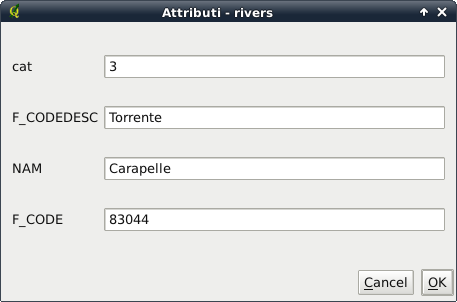
\includegraphics[clip=true, width=8cm]{editDigitizing}
\end{center}
\end{figure}

%\begin{Tip}[ht]\caption{\textsc{Attribute Value Types}}
\begin{Tip}[ht]\caption{\textsc{Types des valeurs d'attribut}}
%\qgistip{At least for shapefile editing the attribue types are validated during the entry. Because of this, it is not possible to enter a number into the text-column in the dialog \dialog{Enter Attribute Values} or vica versa. If you need to do so, you should edit the attributes in a second step within the \dialog{Attribute table} dialog.}
\qgistip{Pour l'\'edition des shapefiles au moins, les types des attributs sont valid\'es au moment de la saisie. \`A cause de cela, il n'est pas possible d'entrer un nombre dans un champ de type texte dans la fen\^etre \dialog{Entrez les valeurs d'attributs} et vice-versa. Si vous avez besoin de le faire, vous devez \'editer les attributs par la suite dans la fen\^etre \dialog{Table d'attributs}.}
\end{Tip}

%\minisec{Move Feature}
%\index{vector layers!move!feature}
\minisec{D\'eplacer des objets}
\index{couches vecteur!d\'eplacer!objet}

%You can move features using the \toolbtntwo{mActionMoveFeature}{Move Feature} icon on the toolbar.
Vous pouvez d\'eplacer des objets en utilisant le bouton \toolbtntwo{mActionMoveFeature}{D\'eplacer Objet} de la barre d'outils.

%\minisec{Split Feature}
%\index{vector layers!split!feature}
\minisec{Couper des objets}
\index{couches vecteur!couper!objet}

%You can split features using the \toolbtntwo{mActionSplitFeatures}{Split Features} icon on the toolbar.
Vous pouvez couper des objets en utilisant le bouton \toolbtntwo{mActionSplitFeatures}{Couper Objet} de la barre d'outils.

%\minisec{Editing Vertices of a Feature}
%\index{vector layers!editing!vertex}
\minisec{\'Editer les sommets d'un objet}
\index{couches vecteur!\'editer!objet}

%For both PostgreSQL/PostGIS and shapefile-based layers, the vertices of features can be edited.
Pour les couches PostgreSQL/PostGIS et shapefile, on peut \'editer les sommets des entit\'es.

%Vertices can be directly edited, that is, you don't have to choose which feature to edit before you can change its geometry. In some cases, several features may share the same vertex and so the following rules apply when the mouse is pressed down near map features:
Les sommets peuvent \^etre \'edit\'es directement, ce qui signifie que vous n'avez pas \`a choisir quelle entit\'e vous voulez \'editer avant que vous puissiez changer sa g\'eom\'etrie. Dans certains cas, plusieurs entit\'es peuvent partager le m\^eme sommet et voil\`a les r\`egles qui s'appliquent lorsqu'un bouton de la souris est press\'e proche d'une entit\'e :

\begin{itemize}
%\item \textbf{Lines}    - The nearest line to the mouse position is used as the target feature. Then (for moving and deleting a vertex) the nearest vertex on that line is the editing target.
\item \textbf{Lignes}    - La ligne la plus proche de la position de la souris est utilis\'ee comme entit\'e cible. Ensuite (pour d\'eplacer ou supprimer un sommet) le sommet le plus proche sur cette ligne est la cible de l'\'edition.
%\item \textbf{Polygons} - If the mouse is inside a polygon, then it is the target feature; otherwise the nearest polygon is used. Then (for moving and deleting a vertex) the nearest vertex on that polygon is the editing target.
\item \textbf{Polygones} - Si la souris est \`a l'int\'erieur d'un polygone, celui-ci est l'entit\'e cibl\'ee ; autrement, le polygone le plus proche est utilis\'e. Ensuite (pour d\'eplacer ou supprimer un sommet) le sommet le plus proche sur ce polygone est la cible de l'\'edition.
\end{itemize}

%You will need to set the property \mainmenuopt{Settings}>\dropmenuopttwo{mActionOptions}{Options}>\tab{Digitizing}>\selectnumber{Search Radius}{10} to a number greater than zero.  Otherwise QGIS will not be able to tell which feature is being edited.
Vous aurez \`a d\'efinir le param\`etre \mainmenuopt{Pr\'ef\'erences}>\dropmenuopttwo{mActionOptions}{Options}>\tab{Num\'erisation}>\selectnumber{Rayon de recherche}{10} \`a un nombre sup\'erieur \`a z\'ero. Sinon QGIS ne sera pas en mesure de dire quelle entit\'e est \'edit\'ee.

%\minisec{Adding Vertices of a Feature}
%\index{vector layers!adding!vertex}
\minisec{Ajouter des sommets \`a un objet}
\index{couches vecteur!ajouter!sommet}

%You can add new vertices to a feature by using the \toolbtntwo{mActionAddVertex}{Add Vertex} icon on the toolbar.
Vous pouvez ajouter de nouveaux sommets en utilisant le bouton \toolbtntwo{mActionAddVertex}{Ajouter un Sommet} de la barre d'outils.

%Note, it doesn't make sense to add more vertices to a Point feature!
Notez qu'il n'y a aucun sens \`a ajouter des sommets \`a des entit\'es de type ponctuelles !

%In this version of QGIS, vertices can only be added to an \textit{existing} line segment of a line feature.  If you want to extend a line beyond its end, you will need to move the terminating vertex first, then add a new vertex where the terminus used to be.
Dans cette version de QGIS, les sommets peuvent uniquement \^etre ajout\'es \`a un segment de ligne \textit{existant}. Si vous voulez \'etendre une ligne au-del\`a de ses extr\'emit\'es, vous devez d'abord d\'eplacer le sommet terminal puis ajouter un nouveau sommet l\`a o\`u le sommet terminal \'etait.

%\minisec{Moving Vertices of a Feature}
%\index{vector layers!moving!vertex}
\minisec{D\'eplacer des sommets d'une entit\'e}
\index{couches vecteur!d\'eplacer!sommet}

%You can move vertices using the \toolbtntwo{mActionMoveVertex}{Move Vertex} icon on the toolbar.
Vous pouvez d\'eplacer des sommets en utilisant le bouton \toolbtntwo{mActionMoveVertex}{D\'eplacer le Sommet} de la barre d'outils.

%\minisec{Deleting Vertices of a Feature}
%\index{vector layers!deleting!vertex}
\minisec{Effacer des sommets d'une entit\'e}
\index{couches vecteur!effacer!sommet}

%You can delete vertices by using the \toolbtntwo{mActionDeleteVertex}{Delete Vertex} icon on the toolbar.
Vous pouvez supprimer des sommets en utilisant le bouton \toolbtntwo{mActionDeleteVertex}{Effacer un Sommet} de la barre d'outils.

%Note, it doesn't make sense to delete the vertex of a Point feature! Delete the whole feature instead.
Notez qu'il n'y a pas de sens \`a supprimer un sommet d'une entit\'e ponctuelle ! Supprimer l'entit\'e compl\`ete \`a la place.

%Similarly, a one-vertex line or a two-vertex polygon is also fairly useless and will lead to unpredictable results elsewhere in QGIS, so don't do that.
De la m\^eme mani\`ere une ligne \`a un sommet ou un polygone \`a deux sommets n'a pas d'int\'er\^et et entra\^inerait des comportements impr\'evisibles dans QGIS, donc ne faites pas \c{c}a. 

%\textbf{Warning:} A vertex is identified for deletion as soon as you click the mouse near an eligible feature. To undo, you will need to toggle Editing off and then discard your changes. (Of course this will mean that other unsaved changes will be lost, too.)
\textbf{Attention :} Un sommet est identifi\'e pour la suppression d\`es que vous cliquer \`a proximit\'e d'une entit\'e. Pour annuler cela, vous devez sortir du mode \'edition sans sauvegarder vos changements. (Bien entendu cela signifie que tous les changements non sauvegard\'es seront perdus).

%\minisec{Add Ring}
%\index{vector layers!add!ring}
\minisec{Ajouter un anneau}
\index{couches vecteur!ajouter!anneau}

%You can create ring polygons using the \toolbtntwo{mActionAddRing}{Add Ring} icon in the toolbar. This means inside an existing area it is possible to digitize further polygons, that will occur as a 'whole', so only the area in between the boundaries of the outer and inner polygons remain as a ring polygon.
Vous pouvez cr\'eez des polygones de type anneau en utilisant le bouton \toolbtntwo{mActionAddRing}{Ajouter Anneau} de la barre d'outils. Ceci signifie qu'il est possible de num\'eriser des polygones \`a l'int\'erieur d'une entit\'e existante, qui seront alors des 'trous' de sorte que seule la zone entre les limites externes et internes du polygone reste, cr\'eant un polygone anneau.


%\minisec{Add Island}
%\index{vector layers!add!island}
\minisec{Ajouter une \^ile}
\index{couches vecteur!ajouter!\^ile}

%You can \toolbtntwo{mActionAddIsland}{add island} polygons to a selected multipolygon. The new island polygon has to be digitized outside the selected multipolygon.
Vous pouvez \toolbtntwo{mActionAddIsland}{Ajouter une \^ile} \`a un multipolygone s\'electionn\'e. Le nouveau polygone \^ile soit \^etre num\'eris\'e en dehors du multipolygone s\'electionn\'e.

%\minisec{Cutting, Copying and Pasting Features}
%\index{vector layers!cut!feature}
%\index{vector layers!copy!feature}
%\index{vector layers!paste!feature}
%\index{editing!cutting features}
%\index{editing!copying features}
%\index{editing!pasting features}
\minisec{Couper, Copier et Coller des entit\'es}
\index{couches vecteur!couper!entit\'e}
\index{couches vecteur!copier!entit\'e}
\index{couches vecteur!coller!entit\'e}
\index{\'editer!couper des entit\'es}
\index{\'editer!copier des entit\'es}
\index{\'editer!coller des entit\'es}

%Selected features can be cut, copied and pasted between layers in the same QGIS project, as long as destination layers are set to  \toolbtntwo{mActionToggleEditing}{Toggle editing} beforehand.
Une entit\'e s\'electionn\'ee peut \^etre coup\'ee, copi\'ee et coll\'ee entre des couches d'un m\^eme projet QGIS, du moment que les couches de destination sont \toolbtntwo{mActionToggleEditing}{Bascul\'ees en mode \'edition} au pr\'ealable.

%Features can also be pasted to external applications as text:  That is, the features are represented in CSV format with the geometry data appearing in the OGC Well-Known Text (WKT) format.
Les entit\'es peuvent \'egalement \^etre coll\'ees dans des applications externes au format texte. Les entit\'es sont alors repr\'esent\'ees au format CSV et leur g\'eom\'etrie appara\^it dans le format OGC Well-Known Text (WKT).

%However in this version of QGIS, text features from outside QGIS cannot  be pasted to a layer within QGIS. When would the copy and paste function come in handy? Well, it turns out that you can edit more than one layer at a time and copy/paste features between layers. Why would we want to do this?  Say we need to do some work on a new layer but only need one or two lakes, not the 5,000 on our \filename{big\_lakes} layer. We can create a new layer and use copy/paste to plop the needed lakes into it.
Cependant, dans cette version de QGIS, les entit\'es au format texte venant d'applications externes ne peuvent pas \^etre coll\'ees \`a une couche dans QGIS. En quoi les fonctions copier et coller sont utiles ? Et bien il se trouve que vous pouvez \'editer plus d'une couche \`a la fois et que vous pouvez alors utiliser les fonctions copier/coller entre les couches. Pourquoi voudrions-nous faire cela ? Imaginons que nous devions travailler sur une nouvelle couche mais que nous avions besoin que d'un ou deux lacs, pas les 5 000 de notre couche \filename{big\_lakes}. Nous pouvons cr\'eer une nouvelle couche puis utiliser copier/coller pour y ins\'erer les quelques lacs.

%As an example we are copying some lakes to a new layer:
Voici un exemple de copie de quelques lacs dans une nouvelle couche :

\begin{enumerate}
%\item Load the layer you want to copy from (source layer)
\item Chargez la couche dont vous voulez copier des entit\'es (couche source)
%\item Load or create the layer you want to copy to (target layer)
\item Chargez ou cr\'eez la couche sur laquelle vous voulez coller des entit\'es (couche cible)
%\item Start editing for target layer
\item Lancez l'\'edition pour la couche cible
%\item Make the source layer active by clicking on it in the legend
\item Assurez-vous que la couche source est active en cliquant dessus dans la l\'egende
%\item Use the \toolbtntwo{mActionSelect}{Select} tool to select the feature(s) on the source layer
\item Utilisez l'outil \toolbtntwo{mActionSelect}{S\'election} pour s\'electionner les entit\'es dans la couche source
%\item Click on the \toolbtntwo{mActionEditCopy}{Copy Features} tool
\item Cliquez sur l'outil \toolbtntwo{mActionEditCopy}{Copier Entit\'es}
%\item Make the destination layer active by clicking on it in the legend
\item Assurez-vous que la couche cible est active en cliquant dessus dans la l\'egende
%\item Click on the \toolbtntwo{mActionEditPaste}{Paste Features} tool
\item Cliquez sur l'outil \toolbtntwo{mActionEditPaste}{Coller Entit\'es}
%\item Stop editing and save the changes
\item Stoppez l'\'edition et sauvegardez les changements
\end{enumerate}

%What happens if the source and target layers have different schemas (field names and types are not the same)? QGIS populates what matches and ignores the rest. If you don't care about the attributes being copied to the target layer, it doesn't matter how you design the fields and data types. If you want to make sure everything - feature and its attributes - gets copied, make sure the schemas match.
Qu'arrive-t-il si les couches source et cible ont diff\'erents sch\'emas de donn\'ees (noms et type des champs diff\'erents) ? QGIS remplit ceux qui correspondent et ignore les autres. Si la copie des attributs ne vous int\'eresse pas, la fa\c{c}on dont vous designer les champs et les types de donn\'ees n'a pas d'importance. Si vous voulez \^etre s\^ur que tout - entit\'e et ses attributs - est copi\'e, assurez-vous que les sch\'emas de donn\'ees correspondent.

%\begin{Tip}[ht]\caption{\textsc{Congruency of Pasted Features}}
\begin{Tip}[ht]\caption{\textsc{Congruence des entit\'es copi\'ees}}
%\qgistip{If your source and destination layers use the same projection, then the pasted features will have geometry identical to the source layer. However if the destination layer is a different projection then QGIS cannot guarantee the geometry is identical. This is simply because there are small rounding-off errors involved when converting between projections.}
\qgistip{Si vos couches source et cible utilisent la m\^eme projection, les entit\'es coll\'ees auront la m\^eme g\'eom\'etrie que dans la couche source. Cependant, si la couche cible n'a pas la m\^eme projection, QGIS ne peut garantir que les g\'eom\'etries seront identiques. Cela est simplement d\^u aux erreurs d'arrondissement faites lors de la conversion de projection.}
\end{Tip}

%\minisec{Deleting Selected Features}
%\index{vector layers!deleting!feature}
\minisec{Supprimer des entit\'es s\'electionn\'ees}
\index{couches vecteur!effacer!entit\'e}

%If we want to delete an entire polygon, we can do that by first selecting the polygon using the regular \toolbtntwo{mActionSelect}{Select Features} tool. You can select multiple features for deletion. Once you have the selection set, use the \toolbtntwo{mActionDeleteSelected}{Delete Selected} tool to delete the features. There is no undo function, but remember your layer isn't really changed until you stop editing and choose to save your changes. So if you make a mistake, you can always cancel the save.
Si nous voulons supprimer un polygone en entier, nous pouvons le faire en s\'electionnant d'abord le polygone en utilisant l'outil \toolbtntwo{mActionSelect}{S\'electionne les donn\'ees}. Vous pouvez s\'electionner plusieurs objets pour la suppression. Une fois le ou les objets s\'electionn\'es, utilisez l'outil \toolbtntwo{mActionDeleteSelected}{Effacer la S\'election} pour les supprimer. Il n'y a pas de fonction annuler mais n'oubliez pas que votre couche n'est r\'eellement chang\'ee tant que vous n'arr\^etez pas l'\'edition et sauvegardez vos changements. Donc si vous faites une erreur, vous pouvez toujours annuler la sauvegarde.

%The \toolbtntwo{mActionEditCut}{Cut Features} tool on the digitizing toolbar can also be used to delete features. This effectively deletes the feature but also places it on a ``spatial clipboard". So we cut the feature to delete. We could then use the \toolbtntwo{mActionEditPaste}{paste tool} to put it back, giving us a one-level undo capability. Cut, copy, and paste work on the currently selected features, meaning we can operate on more than one at a time.
L'outil \toolbtntwo{mActionEditCut}{Couper Entit\'es} de la barre d'outils num\'erisation peut \'egalement \^etre utilis\'e pour supprimer des entit\'es. Ceci supprime effectivement les entit\'es et les place \'egalement dans un ``presse-papier spatial". Donc nous coupons les entit\'es pour les supprimer. Nous pouvons ensuite utiliser l'outil \toolbtntwo{mActionEditPaste}{Coller Entit\'es} pour les r\'ecup\'erer, nous donnant alors la capacit\'e d'annuler une fois les changements. Couper, copier et coller marchent sur les entit\'es s\'electionn\'ees se qui signifie que nous pouvons travailler sur plus d'un objet \`a la fois.

%\begin{Tip}[ht]\caption{\textsc{Feature Deletion Support}}.
\begin{Tip}[ht]\caption{\textsc{Gestion de la suppression d'entit\'es}}
%\qgistip{When editing ESRI shapefiles, the deletion of features only works if QGIS is linked to a GDAL version 1.3.2 or greater. The OS X and Windows versions of QGIS available from the download site are built using GDAL 1.3.2 or higher.}
\qgistip{Lors de l'\'edition de shapefile, la suppression d'entit\'es ne fonctionne que si QGIS est li\'e \`a une version 1.3.2 ou sup\'erieure de GDAL. Les versions OS X et Windows de QGIS disponibles depuis le site de t\'el\'echargement incluent GDAL 1.3.2 ou sup\'erieur.}
\end{Tip}

%\minisec{Snap Mode}
%\index{editing!snap}
\minisec{Mode d'accrochage} 
\index{\'editer!accrochage}
%QGIS allows digitized vertices to be snapped to other vertices of the same layer. To set the snapping tolerance, go to \mainmenuopt{Settings}>\dropmenuopttwo{mActionOptions}{Options}->\tab{Digitizing}. Note that the snapping tolerance is in map units.
QGIS permet aux sommets num\'eris\'es d'\^etre accroch\'es aux autres sommets de la m\^eme couche. Pour d\'efinir la tol\'erance d'accrochage, aller dans \mainmenuopt{Pr\'ef\'erences}>\dropmenuopttwo{mActionOptions}{Options}->\tab{Num\'erisation}. Notez que la tol\'erance d'accrochage est dans les unit\'es de la carte.

%\minisec{Saving Edited Layers}
%\index{editing!saving changes}
\minisec{Sauvegarder les couches \'edit\'ees}
\index{\'editer!sauvegarder des changements}

%When a layer is in editing mode, any changes remain in the memory of QGIS. Therefore they are not committed/saved immediately to the data source or disk. When you turn editing mode off (or quit QGIS for that matter), you are then asked if you want to save your changes or discard them.
Quand une couche est en mode \'edition, tous les changements sont stock\'es en m\'emoire par QGIS. Ils ne sont pas sauvegard\'es imm\'ediatement dans la source de donn\'ees ou sur le disque. Lorsque vous d\'eactivez le mode \'edition (ou quittez QGIS), il vous est demand\'e si vous souhaitez sauvegarder les changements ou les annuler.

%If the changes cannot be saved (e.g. disk full, or the attributes have values that are out of range), the QGIS in-memory state is preserved.  This allows you to adjust your edits and try again.
Si les changements ne peuvent pas \^etre sauv\'es (par exemple \`a cause d'un disque plein ou des valeurs d'attributs d\'epassant la plage pr\'evue), l'\'etat de la m\'emoire de QGIS est pr\'eserv\'e. Cela vous permet d'ajuster vos \'editions et r\'eessayer.

%\subsubsection{Creating a New Layer}\label{sec:create shape}\index{editing!creating a new layer}
\subsubsection{Cr\'eer une nouvelle couche}\label{sec:create shape}\index{\'editer!cr\'eer une nouvelle couche}

%To create a new layer for editing, choose \toolbtntwo{mActionNewVectorLayer}{New Vector Layer} from the \mainmenuopt{Layer} menu. The \dialog{New Vector Layer} dialog will be displayed as shown in Figure \ref{fig:newvectorlayer}. Choose the type of layer (point, line or polygon).
Pour cr\'eer une nouvelle couche \`a \'editer, allez dans \toolbtntwo{mActionNewVectorLayer}{Nouvelle couche vectorielle} du menu \mainmenuopt{Couche}. La fen\^etre \dialog{Nouvelle couche vecteur} apparaitra telle que montr\'ee dans la figure \ref{fig:newvectorlayer}. Choisissez le type de couche (point, ligne ou polygone).

\begin{figure}[ht]
  \begin{center}
  %\caption{Creating a New Vector Dialog \nixcaption}\label{fig:newvectorlayer}\smallskip
  \caption{Fen\^etre Nouvelle couche vecteur \nixcaption}\label{fig:newvectorlayer}\smallskip
  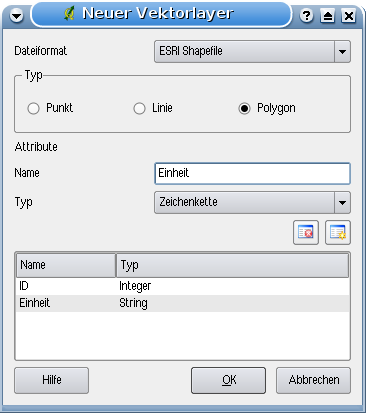
\includegraphics[clip=true, width=10cm]{editNewVector}
\end{center}
\end{figure}

%Note that QGIS does not yet support creation of 2.5D features (i.e. features with X,Y,Z coordinates) or measure features. At this time, only shapefiles can be created. In a future version of QGIS, creation of any OGR or PostgreSQL layer type will be supported.
Notez que QGIS ne g\`ere pas encore la cr\'eation d'entit\'e 2.5D (i.e. des entit\'es avec des coordonn\'ees X, Y, Z). Pour le moment, seuls des shapefiles peuvent \^etre cr\'e\'es. Dans une version future de QGIS, la cr\'eation de n'importe format de couches g\'er\'e par OGR ou PostgreSQL sera possible.

%Creation of GRASS-layers is supported within the GRASS-plugin. Please refer to section \ref{sec:creating_new_grass_vectors} for more information on creating GRASS vector layers.
La cr\'eation de couches GRASS est g\'er\'ee par l'interm\'ediaire de l'extension GRASS. R\'ef\'erez-vous \`a la section \ref{sec:creating_new_grass_vectors} pour plus d'informations sur ce sujet.

%To complete the creation of the new layer, add the desired attributes by clicking on the \button{Add} button and specifying a name and type for the attribute. Only \selectstring{Type}{real}, \selectstring{Type}{integer}, and \selectstring{Type}{string} attributes are supported. Once you are happy with the attributes, click \button{OK} and provide a name for the shapefile. QGIS will automatically add a \filename{.shp} extension to the name you specify.  Once the layer has been created, it will be added to the map and you can edit it in the same way as described in Section \ref{sec:edit_existing_layer} above.
Pour terminer la cr\'eation de la nouvelle couche, ajouter les attributs d\'esir\'es en cliquant sur le bouton \button{Ajouter un attribut} et en sp\'ecifiant le nom et le type de l'attribut. Seuls les attributs de type \selectstring{Type}{r\'eel}, \selectstring{Type}{entier}, et \selectstring{Type}{string} sont g\'er\'es. Une fois satisfait de vos attributs, cliquez sur \button{OK} et donnez un nom pour le shapefile. QGIS va automatiquement ajouter l'extension \filename{.shp} au nom que vous lui avez sp\'ecifi\'e. Une fois la couche cr\'e\'ee, elle sera ajout\'ee \`a la carte et vous pouvez l'\'editer de la mani\`ere d\'ecrite dans la Section \ref{sec:edit_existing_layer} ci-dessus.

%\subsection{Query Builder}\label{sec:query_builder}
\subsection{Constructeur de requ\^etes}\label{sec:query_builder}
%\index{Query Builder}
\index{Constructeur de requ\^etes}

%The Query Builder allows you to define a subset of a table and display it as a layer in QGIS. It can currently only be used with PostGIS layers. For example, if you have a \filename{towns} layer with a \usertext{population} field you could select only larger towns by entering \usertext{population > 100000} in the SQL box of the query builder. Figure \ref{fig:query_builder} shows an example of the query builder populated with data from a PostGIS layer with attributes stored in PostgreSQL.
Le constructeur de requ\^etes vous permet de d\'efinir un sous-ensemble de la table et l'afficher comme une couche dans QGIS. Il peut actuellement \^etre utiliser avec les couches PostGIS. Par exemple, si vous avez une couche \filename{towns} avec un champ \usertext{population}, vous pouvez s\'electionner uniquement les plus grandes villes en entrant \usertext{population > 100000} dans le cadre SQL du constructeur de requ\^ete. La figure \ref{fig:query_builder} montre un exemple de requ\^ete avec les donn\'ees d'une couche PostGIS dont les attributs sont stock\'es dans PostgreSQL.

\begin{figure}[ht]
  \begin{center}
    %\caption{Query Builder \nixcaption}\label{fig:query_builder}\smallskip
    \caption{Constructeur de requ\^etes \nixcaption}\label{fig:query_builder}\smallskip
    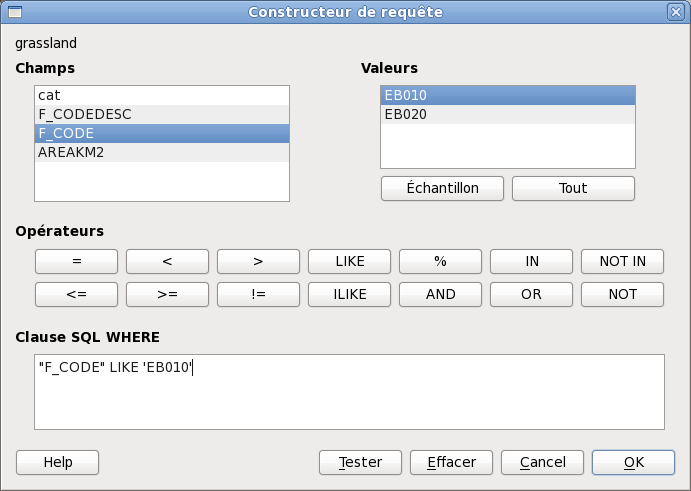
\includegraphics[clip=true, width=11.5cm]{queryBuilder}
  \end{center}
\end{figure}

%The query builder\index{Query Builder} lists the layer's database fields in the list box on the left. You can get a sample of the data contained in the highlighted field by clicking on the \button{Sample} button\index{Query Builder!generating sample list}. This retrieves the first 25 distinct values for the field from the database. To get a list of all possible values for a field, click on the \button{All} button\index{Query Builder!getting all values}. To add a selected field or value to the query, double-click on it\index{Query Builder!adding fields}. You can use the various buttons to construct the query or you can just type it into the SQL box.
Le constructeur de requ\^ete\index{Constructeur de requ\^ete} liste les champs de la couche dans la base de donn\'ees sur la gauche. Vous pouvez obtenir un extrait des donn\'ees contenues dans le champ surlign\'e en cliquant sur le bouton \button{\'Echantillon}\index{Constructeur de requ\^ete!g\'en\'erer une liste d'\'echantillons}. Cela r\'ecup\`ere les 25 premi\`eres valeurs distinctes pour le champ dans la base de donn\'ees. Pour avoir une liste de toutes les valeurs possible dans un champ, cliquez sur le bouton \button{Tout}\index{Constructeur de requ\^ete!obtenir toutes les valeurs}. Pour ajouter un champ ou une valeur s\'electionn\'e \`a la requ\^ete, double-cliquez dessus\index{Constructeur de requ\^ete!ajouter des champs}. Vous pouvez utiliser diff\'erents boutons pour construire une requ\^ete ou vous pouvez simplement taper dans le cadre SQL.

%To test a query, click on the \button{Test} button\index{Query Builder!testing queries}. This will return a count of the number of records that will be included in the layer. When satisfied with the query, click \button{OK}. The SQL for the where clause will be shown in the SQL column of the layer list.
Pour tester une requ\^ete, cliquez sur le bouton \button{Test}\index{Constructeur de requ\^ete!tester des requ\^etes}. Ceci va retourner un compte du nombre d'enregistrements qui seront s\'electionn\'es dans la couche. Une fois satisfait de la requ\^ete, cliquez sur \button{OK}. Le code SQL pour la clause where appara\^itra dans la colonne SQL de la couche.

%\begin{Tip}\caption{\textsc{Changing the Layer Definition}}\index{Query Builder!changing layer definitions}
\begin{Tip}\caption{\textsc{Changer la d\'efinition d'une couche}}\index{Constructeur de requ\^ete!changer des d\'efinitions de couche}
%\qgistip{You can change the layer definition after it is loaded by altering the SQL query used to define the layer. To do this, open the  vector \dialog{Layer Properties} dialog by double-clicking on the layer in the legend and click on the \button{Query Builder} button on the \tab{General} tab. See Section \ref{sec:vectorprops} for more information.}
\qgistip{Vous pouvez changer la d\'efinition d'une couche apr\`es son chargement en modifiant la requ\^ete SQL utilis\'ee pour d\'efinir la couche. Pour faire cela, ouvrez la fen\^etre \dialog{Propri\'et\'es de la couche} en double-cliquant sur la couche dans la l\'egende puis cliquez sur le bouton \button{Constructeur de requ\^ete} dans l'onglet \tab{G\'en\'eral}. Voir Section \ref{sec:vectorprops} pour plus d'informations.}
\end{Tip}

%\subsection{Select by query}\label{sec:select_by_query}
%\index{PostgreSQL!query builder}
%\index{PostGIS!query builder}
%\index{query builder!PostgreSQL}
%\index{query builder!PostGIS}
\subsection{S\'election par requ\^ete}\label{sec:select_by_query}
\index{PostgreSQL!constructeur de requ\^ete}
\index{PostGIS!constructeur de requ\^ete}
\index{constructeur de requ\^ete!PostgreSQL}
\index{constructeur de requ\^ete!PostGIS}

%With QGIS it is possible also to select features using a similar query builder interface to that used in \ref{sec:query_builder}. In the above section the purpose of the query builder is to only show features meeting the filter criteria as a 'virtual layer' / subset. The purpose of the select by query function is to highlight all features that meet a particular criteria. Select by query can be used with all vector data providers.
Dans QGIS, il est possible de s\'electionner des entit\'es en utilisant une interface similaire \`a celle du constructeur de requ\^etes utilis\'e dans \ref{sec:query_builder}. Dans la section ci-dessus, le but du constructeur de requ\^etes \'etait seulement de montrer les entit\'es r\'epondant aux crit\`eres de filtre comme une 'couche virtuelle' / sous-ensemble. Le but de la fonction de s\'election par requ\^ete est de surligner toutes les entit\'es qui r\'epondent \`a un crit\`ere particulier. La s\'election par requ\^ete peut \^etre utilis\'ee sur tous les fournisseurs de donn\'ees vecteur.

%To do a `select by query' on a loaded layer, click on the button \toolbtntwo{mActionOpenTable}{Open Table} to open the attribute table of the layer. Then click the \button{Advanced...} button at the bottom. This starts the Query Builder that allows to define a subset of a table and display it as described in Section \ref{sec:query_builder}.
Pour faire une `s\'election par requ\^ete' sur une couche charg\'ee, cliquez sur le bouton \toolbtntwo{mActionOpenTable}{Ouvrir la table des attributs} pour ouvrir la table de la couche. Ensuite cliquez sur le bouton \button{Avanc\'ee...} en bas de la fen\^etre. Cela lance le Constructeur de requ\^ete qui permet de d\'efinir un sous-ensemble de la table et l'affiche comme d\'ecrit dans la Section \ref{sec:query_builder}.


%\index{vector layers|)}
\index{couches vecteur|)}